\documentclass[11pt,a4paper]{article}

\usepackage{amsmath,amssymb,amsthm}
\usepackage{mathtools}
\usepackage{hyperref}
\usepackage{geometry}
\usepackage{enumitem}
\usepackage{tikz}
\usepackage{tikz-cd}
\usetikzlibrary{arrows.meta,calc,positioning}

\geometry{margin=1in}

\theoremstyle{definition}
\newtheorem{definition}{Definition}[section]
\newtheorem{example}[definition]{Example}
\newtheorem{remark}[definition]{Remark}
\newtheorem{construction}[definition]{Construction}
\newtheorem{notation}[definition]{Notation}
\newtheorem{question}[definition]{Question}

\theoremstyle{plain}
\newtheorem{theorem}[definition]{Theorem}
\newtheorem{lemma}[definition]{Lemma}
\newtheorem{proposition}[definition]{Proposition}
\newtheorem{corollary}[definition]{Corollary}

\newcommand{\R}{\mathbb{R}}
\newcommand{\Z}{\mathbb{Z}}
\newcommand{\F}{\mathbb{F}}
\newcommand{\cF}{\mathcal{F}}
\newcommand{\cE}{\mathcal{E}}
\newcommand{\cB}{\mathcal{B}}
\newcommand{\Prob}{\mathcal{P}}

\title{A Diagrammatic Framework for MPC Protocols: Uniform Description and Information-Geometric Security Analysis}
\author{Research Notes}
\date{December 31, 2025}

\begin{document}

\maketitle

\begin{abstract}
We present a diagrammatic framework for describing and comparing multi-party computation (MPC) protocols in a uniform language. Working in $\mathbf{FinSet}$, we fix an execution object $E=(\prod_i X_i)\times\Omega$ and treat a protocol as a family of morphisms out of $E$. Correctness is expressed as a commuting square: the protocol-induced reconstruction $\rho\circ\pi_S:E\to Y$ agrees with the ideal functionality $f\circ\pi_X:E\to Y$. For security analysis, we extend this base square to an ambient diagram by adjoining observation morphisms $\pi_{\mathrm{full}}:E\to B_{\mathrm{full}}$ and their restrictions $\pi_A:E\to B_A$ for corruption patterns $A$. This ambient diagram serves as an \emph{arrow-translation template}: protocols are compared by instantiating the same pattern of objects and arrows and by analyzing how adversarial observations behave under post-processing. After choosing distributions (e.g.\ sampling protocol randomness and pushing forward along $\pi_A$), the template yields simplex-valued kernels and supports two complementary security layers: Layer~1 compares induced view laws (exactly or approximately, e.g.\ via total variation or KL), while Layer~2 studies posterior structure within feasible fibers determined by inevitable constraints (typically the output). We illustrate the method on Shamir secret sharing, a homomorphic dot-product style protocol (DSDP), and a commodity-server multiplication-sharing primitive (SMC-SPP), emphasizing how corruption growth and protocol post-processing correspond to monotone information refinement via data processing.
\end{abstract}

\tableofcontents

\section{Introduction}

Multi-party computation (MPC) enables parties to compute a function of their private inputs while controlling what information is revealed through an adversary's \emph{view}. While security arguments are often presented in protocol-specific terms (randomness choices, message algebra, simulator constructions), it is useful to have a single methodology that makes heterogeneous protocols comparable under a common description and a common set of leakage diagnostics. We therefore separate two roles. First, an \emph{arrow-translation} template standardizes protocol \emph{representation}: one execution is a point in a total space $E$ (inputs plus randomness), and each corruption pattern $A$ is represented by an observation map $\pi_A:E\to B_A$ (typically as a projection of a maximal transcript), yielding a uniform diagrammatic format across protocols. Second, the language of fibrations together with information-geometric tools standardizes protocol \emph{analysis}: Layer~1 concerns (exact or graded) indistinguishability of induced view laws as points in a probability simplex (e.g.\ collapse or small diameter under TV/KL), while Layer~2 concerns posterior structure within feasible constraint fibers determined by what is inevitably revealed (typically the output). We illustrate this unified workflow in the finite/discrete classical setting on three protocols exhibiting different security requirements and mechanisms.

\subsection{Fundamental MPC View}

We begin with the \emph{correctness} viewpoint of MPC, without introducing any adversary. We work in the category $\mathbf{FinSet}$ (equivalently $\mathbf{Set}$ with all sets finite) and regard the objects in Figure~\ref{fig:protocol-correctness} as sets and the arrows as morphisms. Later, when discussing leakage, we will equip these finite sets with the discrete $\sigma$-algebra and obtain distributions by sampling $\omega\in\Omega$ according to the protocol's randomness model and pushing forward along the relevant observation maps. The space of executions is the product object $E := (\prod_i X_i)\times \Omega$, equipped with the canonical projection $\pi_X:E\to \prod_i X_i$ that forgets randomness. The intended functionality is a morphism $f:\prod_i X_i\to Y$; hence the ``ideal'' output map from executions is the composite $f\circ \pi_X:E\to Y$. A concrete protocol supplies another deterministic morphism $\pi_S:E\to \prod_i S_i$ (full transcript/share vector) together with a reconstruction morphism $\rho:\prod_i S_i\to Y$. Protocol correctness is exactly the statement that these two parallel arrows $E\rightrightarrows Y$ coincide, i.e.\ the square in Figure~\ref{fig:protocol-correctness} commutes:
\[
\rho\circ \pi_S \;=\; f\circ \pi_X.
\]
Equivalently, $\rho$ exhibits $f\circ \pi_X$ as a factorization through $\pi_S$ (no uniqueness is claimed). Section~2 extends this base diagram by adding adversarial observation maps needed for security analysis.

\begin{notation}
We fix the following:
\begin{itemize}
    \item $X_i \subseteq \F_q^{d_i}$: the input space of party $i$, for $i \in \{1, \ldots, n\}$; elements denoted $\chi_i \in X_i$.
    \item $\Omega_i$: the randomness space for party $i$; elements denoted $\omega_i \in \Omega_i$.
    \item $\Omega = \prod_{i=1}^n \Omega_i$: the total randomness space; elements written $\omega = (\omega_1, \ldots, \omega_n)$.
    \item $E = \prod_{i=1}^n X_i \times \Omega$: the total space of protocol states; elements written $(\chi_1, \ldots, \chi_n, \omega)$ or $(\chi, \omega)$ where $\chi = (\chi_1, \ldots, \chi_n)$.
    \item $\pi_X: E \to \prod_{i=1}^n X_i$: the projection forgetting randomness.
    \item $Y$: the output space (codomain of $f$). For concrete protocols over finite fields, $Y = \F_q^k$; other choices include $\Z_m$, $\R$, or $\mathbb{C}$.
    \item $f: \prod_{i=1}^n X_i \to Y$: the function to be securely computed (deterministic in inputs, independent of randomness).
\end{itemize}
\end{notation}

\begin{definition}[Protocol Map]
\label{def:protocol-map}
An $n$-party protocol for computing $f$ consists of:
\begin{enumerate}
    \item A share space $S_i$ for each party $i$.
    \item A protocol map $\pi_S: E \to \prod_{i=1}^n S_i$ assigning shares to each party.
    \item A reconstruction map $\rho: \prod_{i=1}^n S_i \to Y$ such that the diagram in Figure~\ref{fig:protocol-correctness} commutes. That is, $\rho \circ \pi_S = f \circ \pi_X$.
\end{enumerate}
\begin{figure}[ht]
\centering
\begin{tikzcd}
E \arrow[r, "\pi_S"] \arrow[d, "\pi_X"'] & \prod_{i=1}^n S_i \arrow[d, "\rho"] \\
\prod_{i=1}^n X_i \arrow[r, "f"'] & Y
\end{tikzcd}
\caption{Correctness as a commuting square in $\mathbf{FinSet}$: the two composites $E \xrightarrow{\pi_S} \prod_i S_i \xrightarrow{\rho} Y$ and $E \xrightarrow{\pi_X} \prod_i X_i \xrightarrow{f} Y$ coincide.}
\label{fig:protocol-correctness}
\end{figure}
\end{definition}

\subsubsection{Correctness via auxiliary elimination: three categorical mechanisms}
\label{subsubsec:auxiliary-elimination}
Ignoring adversarial views, the correctness square $\rho\circ \pi_S=f\circ \pi_X$ can be read as: a protocol map $\pi_S$ \emph{combines} inputs with auxiliary resources (often denoted $\omega_i$), and reconstruction $\rho$ \emph{cancels} (or quotients out) the auxiliary contribution so that the net effect agrees with the ideal functionality.
This subsection records three common categorical patterns that make this \emph{auxiliary-elimination} intuition mathematically explicit.
\emph{Scope:} these are correctness-side templates only; privacy/leakage requires reintroducing adversarial view arrows in the ambient diagram.

\paragraph{(A) Group-object actions and torsor masking (classical additive-style).}
Assume the base category (here $\mathbf{FinSet}$, but the pattern is more general) has finite products and admits (internal) group objects.
Let $G$ be a group object.
To keep types explicit, assume each share/transcript object $S_i$ carries a right $G$-action and we have a structure map
\[
u_i:\; X_i \longrightarrow S_i,
\]
so that the payload $x_i\in X_i$ is first placed inside the share space and then masked by the $G$-action.
Concretely, fix action morphisms
\[
\beta_i:\; S_i\times G \longrightarrow S_i,
\qquad
(s_i,g)\longmapsto s_i\cdot g.
\]
Let $\omega_i$ be modeled as an element of $G$ (or, more generally, as a point of a $G$-torsor).
Then a basic masking morphism is
\[
\mathrm{mask}_i:\; X_i\times G \longrightarrow S_i,
\qquad
\mathrm{mask}_i(x_i,\omega_i):=u_i(x_i)\cdot \omega_i
\quad\text{(in additive notation: }u_i(x_i)+\omega_i\text{)}.
\]
At the $n$-party level, with $X:=\prod_i X_i$ and $\Omega:=G^n$, one can take $E=X\times \Omega$ and define
\[
\pi_S:=\prod_{i=1}^n \mathrm{mask}_i:\; X\times G^n \longrightarrow \prod_i S_i.
\]
``Cancellation'' is then expressed by requiring $\rho$ to be invariant along the $G$-orbits generated by the masks (or to use algebraic relations among the $\omega_i$ so that the total mask contribution is neutral).
In the simplest additive secret-sharing pattern, one takes $G$ abelian and restricts the auxiliary object to masks whose total product is the identity.
Categorically, rather than taking $\Omega=G^n$, define $\Omega\hookrightarrow G^n$ as the fiber over the identity of the multiplication morphism
\[
\mu:\; G^n \longrightarrow G,
\qquad
(g_1,\dots,g_n)\longmapsto g_1\cdots g_n,
\]
equivalently as the pullback/equalizer of $\mu$ against the unit $e:1\to G$.
In element notation, $(\omega_1,\dots,\omega_n)\in\Omega$ satisfies
\[
\omega_1\cdot \omega_2\cdots \omega_n = e,
\]
so that reconstruction can cancel the total mask contribution.
One categorical way to express cancellation is: $\rho$ factors through the coinvariants/coequalizer of the induced $G$-action on $\prod_i S_i$ (hence is constant on masking orbits).

\paragraph{(B) Monoidal cancellation via duals (evaluation/coevaluation).}
Assume the base category is symmetric monoidal $(\mathcal{C},\otimes,I)$ and \emph{rigid} (every object has a left/right dual).
``Auxiliary resources'' can be modeled by introducing, for each party $i$, a dual pair $(W_i,W_i^\vee)$ with coevaluation and evaluation maps
\[
\mathrm{coev}_i:\; I \longrightarrow W_i\otimes W_i^\vee,
\qquad
\mathrm{ev}_i:\; W_i^\vee\otimes W_i \longrightarrow I,
\]
satisfying the zig--zag (yanking) identities
\[
(\mathrm{id}_{W_i}\otimes \mathrm{ev}_i)\circ (\mathrm{coev}_i\otimes \mathrm{id}_{W_i})=\mathrm{id}_{W_i},
\qquad
(\mathrm{ev}_i\otimes \mathrm{id}_{W_i^\vee})\circ (\mathrm{id}_{W_i^\vee}\otimes \mathrm{coev}_i)=\mathrm{id}_{W_i^\vee}.
\]
An abstract way to formalize ``combine'' is to let the encoding insert a dual pair (or correlate workspaces) and then couple inputs to one side of the pair.
For example, an encoding can have the schematic form
\[
X_i \cong X_i\otimes I
\xrightarrow{\ \mathrm{id}\otimes \mathrm{coev}_i\ }
X_i\otimes W_i\otimes W_i^\vee
\xrightarrow{\ \mathrm{enc}_i\ }
S_i,
\]
where $\mathrm{enc}_i$ is the protocol-specific interaction between the input register and an auxiliary dual pair.
``Cancellation'' is provided when reconstruction composes with $\mathrm{ev}_i$ in a way that matches the inserted $\mathrm{coev}_i$:
the point is not that $\mathrm{ev}_i$ cancels arbitrary ancillas, but that $\mathrm{coev}_i$ followed by $\mathrm{ev}_i$ cancels by the yanking identities when wired compatibly.

\paragraph{(C) Cancellation as quotienting: coequalizers and invariants.}
Assume the base category has the relevant colimits (in particular coequalizers).
Let $\pi_S:E\to S$ be the protocol map (here $S:=\prod_i S_i$).
To say ``$\omega$ does not matter to the decoded output'' can be expressed by identifying an equivalence relation on $S$ generated by varying $\omega$ while keeping the underlying input fixed.
Abstractly, suppose there is a ``masking'' endomorphism (or family of endomorphisms) $m:S\rightrightarrows S$ induced by changing auxiliary degrees of freedom, and form its coequalizer
\[
S \xrightarrow{q} S/{\sim}
\]
so that $q\circ m_1=q\circ m_2$.
Then a cancellation requirement is exactly the existence of a factorization
\[
\rho:\; S \longrightarrow Y
\qquad\text{with}\qquad
\rho=\overline{\rho}\circ q
\]
for some $\overline{\rho}:S/{\sim}\to Y$.
Equivalently: $\rho$ is constant on the identified ``masking'' congruence classes.
There is also a clean formulation directly on the execution side.
Let $X:=\prod_i X_i$ and suppose $\pi_X:E\to X$ presents the ``forget auxiliary'' quotient in the sense that $\pi_X$ is (or is treated as) a coequalizer of its kernel pair:
\[
E\times_X E \rightrightarrows E \xrightarrow{\ \pi_X\ } X.
\]
Then any morphism $h:E\to Y$ that equalizes the two projections $E\times_X E\rightrightarrows E$ factors uniquely through $\pi_X$:
there exists a unique $\bar h:X\to Y$ with $h=\bar h\circ \pi_X$.
Applying this with $h:=\rho\circ \pi_S$ yields $\rho\circ\pi_S=\bar h\circ \pi_X$; correctness is the additional identification $\bar h=f$.

\section{Fibrations and Adversarial Views}

Correctness alone concerns commuting paths from execution space to outputs (Section~1.1). For security analysis, we must also model \emph{partial observations}: which components of an execution become visible to an adversary under a given corruption pattern. Diagrammatically, this means extending the basic correctness square by adjoining explicit view/observation morphisms out of the same total space $E$ (e.g.\ a maximal transcript map and its restrictions to corruption sets). The resulting \emph{ambient diagram} (Figure~\ref{fig:master-diagram}) is what we call the \emph{arrow-translation template}: to compare different protocols, we instantiate the same pattern of arrows (execution $\to$ shares/transcripts $\to$ outputs, and execution $\to$ adversarial views), and then formulate Layer~1/Layer~2 security as properties of the induced view laws and the corresponding fibers/conditionals.

\subsection{Ambient Diagram}

The diagram in Figure~\ref{fig:master-diagram} is the categorical \emph{ambient} diagram that we will instantiate for each protocol. Concretely, we work in $\mathbf{FinSet}$ and interpret each node as an object (a finite set of executions, inputs, transcripts, or views) and each arrow as a morphism (a deterministic map). In particular, by placing all protocol randomness into the execution space $E=(\prod_i X_i)\times \Omega$, the maps $\pi_{\mathrm{full}}$ and $\pi_A$ are honest morphisms in $\mathbf{FinSet}$ rather than stochastic kernels. Probabilistic statements enter only after choosing distributions on the relevant objects (e.g.\ sampling $\omega\in\Omega$ by the protocol's randomness model and pushing forward along $\pi_A$). The same ambient shape can be enriched to non-deterministic or quantum observation models, but here we keep the finite-set, deterministic-arrow setting as the base layer.

\begin{figure}[ht]
\centering
\begin{tikzcd}[row sep={3.0em,between origins}, column sep=huge]
& E
  \arrow[r, "\pi_S"]
  \arrow[d, "\pi_X"']
  \arrow[dl, "\pi_{X_H}"'{pos=0.45}]
  \arrow[rr, bend left=18, "\pi_{\mathrm{full}}"{pos=0.55}]
  \arrow[rrr, bend left=22, "\pi_A"{pos=0.55}]
  \arrow[dr, "\pi_{\mathrm{out}}"{pos=0.35, bend right=20}]
& \prod_{i=1}^n S_i \arrow[d, "\rho"]
& B_{\mathrm{full}}
  \arrow[l, "\mathrm{proj}_S"']
  \arrow[r, "\mathrm{proj}_A"]
  \arrow[dl, "\rho\,\circ\,\mathrm{proj}_S"{pos=0.6}]
& B_A \arrow[l, "\iota_A"', hook, bend left=35]
\\
X_H
& \prod_{i=1}^n X_i \arrow[l, "\mathrm{proj}_{X_H}"] \arrow[r, "f"']
& Y
&
&
\end{tikzcd}
\caption{Ambient diagram (finite-set, deterministic-arrow setting), drawn as an extension of the correctness square in Figure~\ref{fig:protocol-correctness}. In particular, the share map $\pi_S:E\to \prod_i S_i$ remains the top horizontal arrow; additional observation/view maps (to $B_{\mathrm{full}}$ and $B_A$) are attached on the right.}
\label{fig:master-diagram}
\end{figure}

\subsubsection{How to read the ambient diagram}
\label{subsubsec:ambient-diagram-legend}
Section~1.1 already fixes the execution space $E=(\prod_i X_i)\times\Omega$ and the correctness morphisms $\pi_X,\pi_S,\rho,f$.
Here we record the conventions and objects used to interpret adversarial views and post-processing in Figure~\ref{fig:master-diagram}.

\textbf{Adversarial conventions.}
\begin{itemize}
    \item $A \subseteq \{1, \ldots, n\}$: the set of corrupted (adversarial) parties, and $H = \{1, \ldots, n\} \setminus A$ the set of honest parties.
    \item $X_H := \prod_{i \in H} X_i$ and $X_A := \prod_{i \in A} X_i$, with $\mathrm{proj}_{X_H}: \prod_{i=1}^n X_i \to X_H$ the projection forgetting adversarial inputs.
    \item \textbf{Probability Context:} protocol randomness $\omega\in\Omega$ is sampled from its specified distribution (uniform in the finite-field setting). For Layer~2 statements involving posteriors on inputs, we use a uniform prior on $\prod_i X_i$ as a maximum-entropy leakage test.
    \begin{itemize}
        \item This does \emph{not} imply real-world inputs must be uniform.
        \item Rather, a uniform prior isolates whether the protocol induces any bias beyond the constraint geometry (fibers).
    \end{itemize}
\end{itemize}

\textbf{View objects.}
\begin{itemize}
    \item $B_{\mathrm{full}}$: full (counterfactual) observation space. In the finite classical model one can take $B_{\mathrm{full}}=\prod_i S_i\times \prod_i X_i$.
    \item $B_A$: adversary view space. In the finite classical model one can take $B_A=\prod_{i\in A}S_i\times \prod_{i\in A}X_i$.
\end{itemize}

\textbf{View maps (observation morphisms).}
\begin{itemize}
    \item $\pi_{\mathrm{full}}: E \to B_{\mathrm{full}}$: maximal transcript / full observation map (Definition~\ref{def:full-fibration}).
    \item $\pi_A:E\to B_A$: adversarial view map obtained by restricting $\pi_{\mathrm{full}}$ to the coordinates visible to $A$.
\end{itemize}

\textbf{Post-processing maps.}
\begin{itemize}
    \item $\mathrm{proj}_S: B_{\mathrm{full}} \to \prod_i S_i$: projection to shares.
    \item $\mathrm{proj}_A: B_{\mathrm{full}} \to B_A$: projection to the adversary's classical coordinates (public transcript + corrupted classical locals, etc.).
    \item $\iota_A: B_A \hookrightarrow B_{\mathrm{full}}$: inclusion of adversary's view into full view (padding inclusion; non-operational).
\end{itemize}

\textbf{Commutativity relations (as read off from Figure~\ref{fig:master-diagram}).}
\begin{enumerate}
    \item $\rho \circ \pi_S = f \circ \pi_X$ (protocol correctness).
    \item $\pi_{\mathrm{out}} = f \circ \pi_X = \rho \circ \pi_S$ (output = reconstruction of shares).
    \item $\pi_A = \mathrm{proj}_A \circ \pi_{\mathrm{full}}$ (adversarial view is restriction of full view).
\end{enumerate}

\paragraph{Information lens (partitions induced by observations).}
The ambient diagram lives in $\mathbf{FinSet}$ and records \emph{operational} observation maps $\pi:E\to B$.
To make ``information growth'' precise (and to support cofibration-like language as \emph{inclusions of information}), it is convenient to pass to the \emph{partition of executions} induced by an observation map.
Given $\pi:E\to B$, define the equivalence relation $e\sim_\pi e'$ iff $\pi(e)=\pi(e')$, and write
\[
\Pi(\pi)\ :=\ \{\,\pi^{-1}(b)\subseteq E:\ b\in \mathrm{im}(\pi)\,\}
\]
for the corresponding partition of $E$ into $\pi$-fibers.
Post-processing corresponds to partition coarsening: if $\pi_1=q\circ \pi_2$ for some $q$, then $\Pi(\pi_2)$ refines $\Pi(\pi_1)$.
In particular, $\pi_A=\mathrm{proj}_A\circ \pi_{\mathrm{full}}$ implies $\Pi(\pi_{\mathrm{full}})$ refines $\Pi(\pi_A)$.

\begin{figure}[ht]
\centering
\begin{tikzcd}[row sep=large, column sep=huge]
E \arrow[r, "\pi_{\mathrm{full}}"] \arrow[dr, "\pi_A"'] & B_{\mathrm{full}} \arrow[d, "\mathrm{proj}_A"] \\
& B_A
\end{tikzcd}

\vspace{0.5em}

\begin{tikzcd}[row sep=large, column sep=huge]
\Pi(\pi_{\mathrm{full}}) \arrow[r, "\text{coarsen / forget}"] & \Pi(\pi_A)
\end{tikzcd}
\caption{Derived ``information layer'' under the ambient diagram: each deterministic observation $\pi:E\to B$ induces a partition $\Pi(\pi)$ of executions into indistinguishability classes. Post-processing (forgetting coordinates) coarsens partitions; equivalently, larger views correspond to partition refinements.}
\label{fig:master-diagram-partition-lens}
\end{figure}

\section{Fibrations as Observation Maps}
\label{sec:fibrations-as-observation-maps}
We distinguish notions of observation that correspond to different maps $\pi:E\to B$, with different fiber and posterior structure.

\begin{definition}[Fiber]
\label{def:fiber}
For a map $\pi: E \to B$ and a point $b \in B$, the \textbf{fiber} over $b$ is the preimage
\[
\cF_b := \pi^{-1}(b) = \{ e \in E : \pi(e) = b \} \subseteq E.
\]
\end{definition}

\begin{definition}[Probability Simplex on a Finite Set]
\label{def:prob-simplex}
Let $S$ be a finite set. The probability simplex on $S$ is
\begin{equation}
\label{eq:prob-simplex}
\Prob(S)\ :=\ \Bigl\{\,p:S\to[0,1]\ \Bigm|\ \sum_{s\in S} p(s)=1\,\Bigr\}.
\end{equation}
Equivalently, if $|S|=m$ and $S=\{s_1,\dots,s_m\}$, then $\Prob(S)$ identifies with the standard simplex
$\Delta^{m-1}\subseteq\mathbb{R}^m$ via $p\mapsto (p(s_1),\dots,p(s_m))$.
We also write $\delta_S:S\to\Prob(S)$ for the \emph{Dirac embedding}, $\delta_S(s)=\delta_s$.
\end{definition}

\noindent \textbf{Section roadmap.} From this point onward, we organize the analysis around a small collection of deterministic maps out of the execution space $E$ (coordinate projections onto inputs/honest coordinates, protocol share/transcript maps, output maps, and adversarial view maps). These maps provide the common ``fiber language'' reused later for both view-law geometry (Layer~1) and posterior-on-fibers analysis (Layer~2).

\paragraph{Terminology (``fibration'' as an observation-map analogue).}
In what follows we use the word \emph{fibration} in an \emph{analogical} sense: a ``fibration'' is simply a deterministic observation/projection map $\pi:E\to B$ together with its induced fiber partition $\{\pi^{-1}(b)\}$ and (after fixing a prior) its pushforward law and conditional posteriors (Definition~\ref{def:statistical-fibration}).
We do \emph{not} assume any Serre/Grothendieck/Quillen lifting axioms, nor do we fix a model structure on $\mathbf{FinSet}$.
The benefit of the term is organizational: it lets us speak uniformly about (i) fibers as indistinguishability classes, and (ii) how post-processing and corruption growth correspond to monotone information refinement (Figure~\ref{fig:master-diagram-partition-lens}).

\begin{definition}[Statistical fibration / disintegration (finite/discrete version)]
\label{def:statistical-fibration}
Let $\pi:E\to B$ be a map of finite sets, and let $\mu\in\Prob(E)$ be a prior on $E$.
Write $\nu := \pi_*\mu \in \Prob(B)$ for the \textbf{pushforward} (the law of the observation $\pi(e)$ when $e\sim\mu$), i.e.
\[
\nu(b)=\mu\!\bigl(\pi^{-1}(b)\bigr)=\sum_{e\in E:\,\pi(e)=b}\mu(e).
\]
Equivalently, $\pi$ induces a map $\pi_*:\Prob(E)\to\Prob(B)$ on simplices; it is characterized by commutativity with the Dirac embeddings $\delta_E,\delta_B$:
\[
\begin{tikzcd}
E \arrow[r, "\pi"] \arrow[d, "\delta_E"'] & B \arrow[d, "\delta_B"] \\
\Prob(E) \arrow[r, "\pi_*"'] & \Prob(B).
\end{tikzcd}
\]
For each $b\in B$ with $\nu(b)>0$, define the \textbf{fiber (posterior) measure} $\mu_b\in\Prob(E)$ by
\[
\mu_b(e)
\ :=\
\begin{cases}
\mu(e)/\nu(b), & \text{if }\pi(e)=b,\\
0, & \text{otherwise.}
\end{cases}
\]
Then $\mu_b$ is supported on the fiber $\cF_b=\pi^{-1}(b)$ and satisfies the discrete disintegration identity
\[
\mu(e)\ =\ \sum_{b\in B}\nu(b)\,\mu_b(e).
\]
Equivalently, $b\mapsto \mu_b$ is the conditional law (regular conditional distribution) of $e$ given the observation $\pi(e)=b$ in the finite/discrete setting.
\end{definition}

\paragraph{Probabilistic Semantics (Priors, Pushforward, Posteriors).}
\label{par:probabilistic-semantics}
In this note, the observation maps $\pi:E\to B$ are deterministic arrows, and probability enters only through a prior $\mu\in\Prob(E)$.
Unless stated otherwise, we use a product prior $\mu=\mu_X\times \mu_\Omega$, where $\mu_\Omega$ is uniform on protocol randomness and $\mu_X$ is a chosen prior on inputs (often uniform for baseline leakage diagnostics).
For such a prior, the pushforward $\nu=\pi_*\mu\in\Prob(B)$ is the law of the observable transcript/view, and the conditional measures $\mu_b$ from Definition~\ref{def:statistical-fibration} are the corresponding posteriors on hidden coordinates given the observation $b$.

\paragraph{From the Abstract Setup to Protocol-Specific Observation Maps.}
We now specialize the abstract observation picture to the concrete morphisms that appear in MPC.
Each subsequent definition fixes a particular map $\pi:E\to B$ (input projections, share map, output observation, and view/transcript observations), so that one can speak uniformly about its fibers $\pi^{-1}(b)$ and---after choosing a prior $\mu$---about induced laws $\pi_*\mu$ and posteriors on the corresponding fibers.
This separates \emph{structural} coordinate projections (available from the product decomposition of $E$) from \emph{operational} observation maps that model what a protocol or adversary actually records.

\subsection{Coordinate Projections and Share Map}

\subsubsection{Input Fibration}
\begin{definition}[Input Fibration]
\label{def:input-fibration}
The \textbf{input fibration} is the map
\[
\pi_X: E \longrightarrow \prod_{i=1}^n X_i
\]
defined by $\pi_X(\chi, \omega) = \chi$. This map defines a \textbf{trivial fiber bundle} because the total space $E$ is globally isomorphic to the product of the base space $\prod X_i$ and the fiber $\Omega$. The fiber over any input $\chi$ is simply the entire randomness space:
\[
\pi_X^{-1}(\chi) = \{\chi\} \times \Omega \cong \Omega.
\]
Geometrically, this means the randomness is independent of the inputs.
\end{definition}

\subsubsection{Honest-Input Coordinate Projection}
\begin{definition}[Honest-Input Coordinate Projection]
\label{def:honest-input-fibration}
The \textbf{honest-input coordinate projection} is the map
\[
\pi_{X_H}: E \longrightarrow X_H
\]
defined by
\[
\pi_{X_H} := \mathrm{proj}_{X_H} \circ \pi_X,
\]
where $\mathrm{proj}_{X_H}: \prod_{i=1}^n X_i \to X_H$ forgets adversarial inputs.

This is a \emph{structural} (non-operational) map: it does not correspond to an observation from protocol execution, but is induced by the product decomposition of the global state space.

In our product model $E = \bigl(\prod_i X_i\bigr)\times \Omega$, this is again a (trivial) projection. The fiber over an honest input $\chi_H \in X_H$ is
\[
\pi_{X_H}^{-1}(\chi_H)
:= \{(\chi,\omega)\in E : \mathrm{proj}_{X_H}(\chi)=\chi_H\}
:= \bigl(\{\chi_H\}\times X_A\bigr)\times \Omega.
\]
\end{definition}

\paragraph{Structural vs.\ statistical independence.}
The condition that $\pi_X$ is a \emph{trivial} bundle corresponds to \textbf{structural independence}: the space of available randomness $\Omega$ is the same for every input and can be defined globally.
This is distinct from \emph{statistical independence} of random variables under the prior $\mu$ (Paragraph~\ref{par:probabilistic-semantics}).
In standard MPC, we construct $E$ as a product $X\times \Omega$, ensuring this structural independence by definition.

\paragraph{Independent choice of inputs (product structure).}
In standard MPC, \textbf{parties choose their inputs independently}:
\begin{itemize}
    \item Alice picks $\chi_A \in X_A$ without knowing Bob's input.
    \item Bob picks $\chi_B \in X_B$ without knowing Alice's input.
    \item The total input space is the \textbf{product} $\prod_i X_i$, reflecting this independence.
\end{itemize}
The protocol $\pi_S$ then creates relationships on \emph{shares and outputs}, but these are consequences of how the protocol processes independent inputs---not prior constraints requiring coordination between parties.

Non-trivial geometry of $X_i$ typically arises from \textbf{per-party data type constraints} (e.g., normalized vectors, probability distributions), not from cross-party coordination. Cross-party input constraints would require unusual settings like trusted setup or verifiable computation.

\paragraph{Inputs as parameters (examples).}
The geometric perspective suggests a generalization: inputs need not be ``data'' in the traditional sense (numbers, strings) but can be \textbf{parameters} that configure the computation:
\begin{itemize}
    \item \textbf{Federated Learning:} Inputs are model gradients (vectors with norm constraints) $\to$ $X_i \subseteq S^{n-1}$ or a ball.
    \item \textbf{Secure Voting:} Inputs are preference distributions $\to$ $X_i = \Delta^k$ (simplex).
    \item \textbf{Secure Robotics:} Inputs are orientations or poses $\to$ $X_i = SO(3)$ or $SE(3)$.
\end{itemize}
This reveals that MPC naturally extends to settings where the ``secrets'' are geometric or parametric objects, not just field elements.

\subsubsection{Share Fibration}
\begin{definition}[Share Fibration]
\label{def:share-fibration}
The \textbf{share fibration} is the protocol map
\[
\pi_S: E \longrightarrow \prod_{i=1}^n S_i
\]
which assigns shares to each party. The fiber over a share tuple $s = (s_1, \ldots, s_n)$ is:
\[
\pi_S^{-1}(s) = \{(\chi, \omega) \in E : \pi_S(\chi, \omega) = s\}.
\]
This fiber contains all protocol states (input-randomness pairs) that produce the same shares. Unlike the input fibration, this fiber generally contains \emph{multiple inputs}---different inputs can produce the same shares when paired with appropriate randomness. This is the essence of security: the shares do not uniquely determine the inputs.
\end{definition}

\subsection{The Output Observation}

The \textbf{output observation} captures the scenario where all shares are observed, randomness terms cancel, and the function output $f(\chi)$ is revealed---but the individual inputs are not directly observed.

\subsubsection{Output Observation Map}
\begin{definition}[Output Observation]
\label{def:output-fibration}
The \textbf{output observation map} is
\[
\pi_{\mathrm{out}}: E \longrightarrow Y
\]
defined by $\pi_{\mathrm{out}}(\chi, \omega) = f(\chi)$, where $f: \prod_{i=1}^n X_i \to Y$ is the function being computed.
\end{definition}

\begin{proposition}[Randomness cancellation / correctness]
\label{prop:randomness-cancellation}
Assume protocol correctness $\rho \circ \pi_S = f \circ \pi_X$.
Then the reconstruction $\rho$ applied to the share tuple $\pi_S(\chi,\omega)$ depends only on the input $\chi$ and equals the intended output $f(\chi)$; in particular, the protocol randomness $\omega$ is \emph{invisible} at the output level.
\end{proposition}
\begin{proof}
For any $(\chi,\omega)\in E$, we have
\[
\rho(\pi_S(\chi,\omega))=(\rho\circ \pi_S)(\chi,\omega)=(f\circ \pi_X)(\chi,\omega)=f(\chi),
\]
which does not depend on $\omega$.
\end{proof}

\begin{proposition}[Fiber Structure of Output Fibration]
\label{prop:output-fiber}
For $b \in Y$, the fiber of the output fibration is
\[
\cF_b := \pi_{\mathrm{out}}^{-1}(b) = f^{-1}(b) \times \Omega = \{(\chi, \omega) : f(\chi) = b\}.
\]
This fiber contains \textbf{all input combinations} $\chi$ that yield output $b$, paired with all possible randomness values.
\end{proposition}

\begin{example}[Scalar Product]
Consider the scalar product $f(x_1, x_2) = x_1 \cdot x_2$ over $\F_q$. Suppose the protocol computes shares $y_1, y_2$ such that $y_1 + y_2 = x_1 \cdot x_2$.

Observing both shares $(y_1, y_2)$ reveals the product $b = y_1 + y_2 = x_1 \cdot x_2$. The fiber over $b$ is:
\[
\cF_b = \{(x_1, x_2) \in \F_q^2 : x_1 \cdot x_2 = b\} \times \Omega.
\]
This is a \textbf{hyperbola} in $\F_q^2$:
\begin{itemize}
    \item If $b \neq 0$: the fiber contains $q - 1$ input pairs (excluding $x_1 = 0$ or $x_2 = 0$).
    \item If $b = 0$: the fiber contains $2q - 1$ input pairs (the axes $x_1 = 0$ or $x_2 = 0$).
\end{itemize}
Thus, knowing the output does \emph{not} determine the individual inputs.
\end{example}

\subsection{The Full Observation}

The \textbf{full observation} represents the scenario where all shares \emph{and} all inputs are directly observed. This is a stronger observation model.

\subsubsection{Full Observation Space}
\begin{definition}[Full Observation Space]
The \textbf{full observation space} is
\[
B_{\mathrm{full}} := \prod_{i=1}^n S_i \times \prod_{i=1}^n X_i,
\]
consisting of all shares and all inputs.
\end{definition}

\subsubsection{Full Observation Map}
\begin{definition}[Full Observation]
\label{def:full-fibration}
The \textbf{full observation map} is
\[
\pi_{\mathrm{full}}: E \longrightarrow B_{\mathrm{full}}
\]
defined by $\pi_{\mathrm{full}}(\chi_1, \ldots, \chi_n, \omega) = \bigl( (\pi_S(\chi, \omega))_{i=1}^n, (\chi_i)_{i=1}^n \bigr)$.
\end{definition}

\begin{proposition}[Fiber of the full observation]
\label{prop:fiber-full-observation}
For $b=(s,\chi)\in B_{\mathrm{full}}$, the fiber $\pi_{\mathrm{full}}^{-1}(b)$ consists exactly of those randomness values $\omega$ that produce the share tuple $s$ on input $\chi$:
\[
\pi_{\mathrm{full}}^{-1}(s,\chi)=\{(\chi,\omega)\in E:\pi_S(\chi,\omega)=s\}
\ \cong\ \{\omega \in \Omega : \pi_S(\chi, \omega) = s\}.
\]
\end{proposition}

\subsection{Comparison of Global Fibrations}

\begin{center}
\begin{tabular}{l|c|c}
& \textbf{Output Fibration} $\pi_{\mathrm{out}}$ & \textbf{Full Observation} $\pi_{\mathrm{full}}$ \\
\hline
Base space & $Y$ (function output) & $\prod_i S_i \times \prod_i X_i$ \\
What's observed & Output $f(\chi)$ & All shares + all inputs \\
Fiber $\cF_b$ contains & All $(\chi, \omega)$ with $f(\chi) = b$ & Only compatible $\omega$ \\
Inputs in fiber? & Yes (multiple) & No (fixed by observation) \\
Randomness in fiber? & Yes (all of $\Omega$) & Possibly unique \\
\end{tabular}
\end{center}

\begin{proposition}[Factorization of the output observation]
\label{prop:output-factorization}
The output observation factors as $\pi_{\mathrm{out}} = f\circ \pi_X$.
\begin{figure}[ht]
\centering
\begin{tikzcd}
E \arrow[r, "\pi_X"] \arrow[dr, "\pi_{\mathrm{out}}"'] & \prod_{i=1}^n X_i \arrow[d, "f"] \\
& Y
\end{tikzcd}
\caption{Output fibration factors through input projection.}
\label{fig:output-factorization}
\end{figure}
\end{proposition}

\subsection{The Adversarial Observation}

\subsubsection{Adversarial Observation Space}
\begin{definition}[Adversarial Observation Space]
Let $t$ with $0 \leq t < n$ be the corruption threshold (the number of corrupted parties). Let $A \subseteq \{1, \ldots, n\}$ with $|A| = t$ be the set of corrupted parties. The \textbf{adversarial observation space} is
\[
B_A := \prod_{i \in A} S_i \times \prod_{i \in A} X_i,
\]
consisting of the shares and inputs visible to the adversary.
\end{definition}

\subsubsection{Adversarial Observation Map}
\begin{definition}[Adversarial Observation]
\label{def:adv-fibration}
The \textbf{adversarial observation map} is
\[
\pi_A: E \longrightarrow B_A
\]
defined by $\pi_A(\chi_1, \ldots, \chi_n, \omega) = \bigl( (\pi_S(\chi, \omega))_{i \in A}, (\chi_i)_{i \in A} \bigr)$.
\end{definition}

\begin{lemma}[Adversarial view as restriction of the full view]
\label{lem:adv-as-restriction}
Let $\mathrm{proj}_A: B_{\mathrm{full}} \to B_A$ be the coordinate projection that restricts to the adversary's coordinates. Then
\[
\pi_A = \mathrm{proj}_A \circ \pi_{\mathrm{full}}.
\]
\end{lemma}

\paragraph{Realizable adversarial views (image of $\pi_A$).}
The space $B_A = \prod_{i \in A} S_i \times \prod_{i \in A} X_i$ is an ambient product of coordinates visible to $A$.
Not every $b\in B_A$ must be realizable by the protocol, so $\pi_A$ need not be surjective.
When discussing fibers $\pi_A^{-1}(b)$, we implicitly restrict to $b\in \mathrm{im}(\pi_A)$.

\begin{notation}[Fiber over Adversarial View]
For $b \in B_A$, we write $\cF_b := \pi_A^{-1}(b)$ for the fiber over $b$ (Definition~\ref{def:fiber}). This consists of all protocol states consistent with the adversary's observation $b$. Security is characterized by fiber properties.
\end{notation}

\subsection{The Honest Projection}

\begin{notation}
Let $H = \{1, \ldots, n\} \setminus A$ denote the set of honest parties. Define:
\[
X_H := \prod_{i \in H} X_i, \qquad X_A := \prod_{i \in A} X_i.
\]
\end{notation}

\subsubsection{Honest Projection of an Adversarial Fiber}
\begin{definition}[Honest Projection of an Adversarial Fiber]
\label{def:honest-component}
For a fiber $\cF_b=\pi_A^{-1}(b)\subseteq E$ over adversarial view $b = (s_A, \chi_A)$, the \textbf{honest projection} is its image under the coordinate projection $E\to X_H\times\Omega$, namely
\[
\cF_b^H := \mathrm{proj}_{X_H \times \Omega}(\cF_b) \subseteq X_H \times \Omega.
\]
This is the set of honest inputs and randomness values compatible with observation $b$,
which represents the \emph{secret information} that the protocol
aims to protect from the adversary. For a protocol to be secure,
all elements of $\cF_b^H$ should be equally likely given the adversary's observation $b$
---this is the ``uniform on the fiber'' intuition behind Layer~2 input-hiding.
\end{definition}

\paragraph{Geometric Structure of $\cF_b^H$.}
Its geometric structure is protocol-dependent;
see Section~\ref{sec:bridge-to-analysis}
(especially the subsection on protocol-dependent geometry)
for the taxonomy used in later analyses.

\section{Bridge to Quantitative Analysis: From Fibers to View Laws}
\label{sec:bridge-to-analysis}

Section~\ref{sec:fibrations-as-observation-maps} is intentionally formal and uniform: it fixes the
execution space $E$, observation maps $\pi:E\to B$, and the induced fiber picture of
indistinguishability.
To proceed toward \emph{security analysis}, we connect this fiber language to
(i) probability laws of what an adversary sees, and (ii) quantitative notions of
distinguishability (divergences, metrics, monotone growth under post-processing).

\subsection{Operational Observations vs.\ Coordinate Projections}
Some maps $\pi:E\to B$ model \emph{operational} views arising from execution
(e.g.\ the adversarial observation $\pi_A$), while others are \emph{coordinate projections}
used to specify which coordinates are treated as secrets (e.g.\ $\pi_{X_H}$).
Both are legitimate in the diagrammatic viewpoint: security asks how operational observations
reshape the posterior on designated secret coordinates.

\subsection{Protocol-Dependent Geometry of the Honest Projection \texorpdfstring{$\cF_b^H$}{F_b^H}}
Fix an adversarial view value $b\in B_A$ and consider the remaining feasible set of honest
coordinates (the honest projection of the fiber)
\[
\cF_b^H \subseteq X_H\times \Omega.
\]
This set is the basic ``residual uncertainty object'' on which later analyses operate.
Its \emph{mathematical structure} is not universal: it is determined by the structure of the \emph{protocol maps} (in particular the observation/view maps such as $\pi_A$ and $\pi_S$ that implement the target functionality $f$), together with the chosen modeling regime (finite-field/linear, algebraic, smooth approximation, etc.).
The function $f$ controls the output constraint (the output fiber of $\pi_{\mathrm{out}}$), but the geometry of $\cF_b^H$ reflects how the protocol realizes $f$ at the level of views.
For example:
\begin{itemize}
\item \textbf{Linear protocols:} $\cF_b^H$ is typically an affine subspace; linear algebra controls size/dimension.
\item \textbf{Polynomial-based protocols:} $\cF_b^H$ becomes an algebraic set; degree/variety structure matters.
\item \textbf{Smooth/continuous relaxations:} $\cF_b^H$ may be modeled as a submanifold; differential tools become available.
\end{itemize}
Accordingly, the framework does not aim to classify $\cF_b^H$ in full generality; rather, this
is the point where one \emph{instantiates} the framework for a given protocol.

\subsection{From a Deterministic View Map to a Point in a Simplex (the Simplex-Map Lens)}
To quantify leakage, one passes from set-valued fibers to \emph{distributions of views} by fixing a prior on protocol randomness (and optionally on inputs) and then pushing it forward along the deterministic view map.
Concretely, after fixing adversarial inputs $\chi_A$ one obtains a deterministic map on the slice $X_H\times \Omega \to S_A$, and hence a law-valued map into the simplex $\Prob(S_A)$ (Definition~\ref{def:prob-simplex}).
\[
K^{(A,\chi_A)}:X_H \to \Prob(S_A),\qquad \chi_H\mapsto \mathrm{Law}(V_A\mid \chi_A,\chi_H),
\]
whose image lies in the probability simplex $\Prob(S_A)$.

\paragraph{Optional: Mutual-Information Leakage Under an Input Prior.}
The simplex-valued map $K^{(A,\chi_A)}$ is a kernel (Markov kernel / stochastic map), i.e.\ it assigns to each $\chi_H\in X_H$ a distribution $K^{(A,\chi_A)}(\chi_H)\in\Prob(S_A)$.
To obtain an information-theoretic leakage scalar, one may also choose a prior $\mu_{X_H}\in\Prob(X_H)$ on honest inputs (keeping $\chi_A$ fixed), inducing a joint distribution on $(\chi_H,V_A)$ via
\[
\chi_H\sim \mu_{X_H},\qquad V_A \mid \chi_H \sim K^{(A,\chi_A)}(\chi_H).
\]
In the finite/discrete setting, the corresponding mutual information can be written as
\[
I(\chi_H;V_A\mid \chi_A)
\;=\;
\sum_{\chi_H\in X_H}\mu_{X_H}(\chi_H)\,
D_{\mathrm{KL}}\!\Bigl(K^{(A,\chi_A)}(\chi_H)\,\Big\|\,\sum_{\chi_H'\in X_H}\mu_{X_H}(\chi_H')\,K^{(A,\chi_A)}(\chi_H')\Bigr).
\]
Perfect output-hiding corresponds to $K^{(A,\chi_A)}$ being constant; graded leakage is measured
by the diameter of its image under a chosen divergence/metric (e.g.\ total variation, KL, Fisher--Rao in smooth families).

\subsection{Roadmap for the Next Analysis Sections}
The subsequent analysis parts will build on the bridge above:
\begin{itemize}
\item \textbf{Layered security statements:} express Layer~1 and Layer~2 as constraints on induced view laws and posteriors.
\item \textbf{Monotone information growth:} model rounds/corruption/coarsening via post-processing maps and chains of views.
\item \textbf{Information geometry:} study families of view laws inside $\Prob(S_A)$ using KL/Fisher and related projection principles.
\end{itemize}

\section{Layered Security: Output-Hiding and Input-Hiding}
\label{sec:layered-security}
We now record the two baseline security notions used throughout the later analysis: Layer~1 (\textbf{Output-Hiding}, expressed as indistinguishability of induced view laws) and Layer~2 (\textbf{Input-Hiding}, expressed as a posterior flatness condition once inevitable constraints are fixed).

\subsection{Layer 1: Output-Hiding via View Laws}
Fix a corruption set $A$ and an adversarial input $\chi_A\in X_A$.
Write $S_A:=\prod_{i\in A}S_i$ for the shares-only view alphabet and let
\[
\jmath_{\chi_A}:X_H\times \Omega\to E,\qquad (\chi_H,\omega)\longmapsto (\chi_A,\chi_H,\omega)
\]
denote the honest-slice embedding.
Let $\mathrm{proj}_{S_A}:B_A\to S_A$ be the coordinate projection onto the shares component, and define the deterministic shares-view map
\[
\Phi_{\chi_A}\ :=\ \mathrm{proj}_{S_A}\circ \pi_A\circ \jmath_{\chi_A}:\ X_H\times \Omega\to S_A.
\]
Also write $f_{\chi_A}:X_H\to Y$ for the partial evaluation $f_{\chi_A}(\chi_H):=f(\chi_A,\chi_H)$.

\paragraph{Commutative relations induced by slicing.}
The slice embedding $\jmath_{\chi_A}$ restricts the ambient arrows in Figure~\ref{fig:master-diagram} to maps on $X_H\times\Omega$. It induces the shares-view map $\Phi_{\chi_A}$, and it also makes explicit that the output map \emph{factors through} the projection $\mathrm{proj}_{X_H}:X_H\times\Omega\to X_H$ (hence does not depend on $\omega$):
\begin{figure}[ht]
\centering
\begin{tikzcd}[column sep=large, row sep=large]
X_H\times \Omega
\arrow[r, "\jmath_{\chi_A}"]
\arrow[d, "\mathrm{proj}_{X_H}"']
\arrow[rrd, "\Phi_{\chi_A}"', pos=0.25]
& E
\arrow[r, "\pi_A"]
\arrow[d, "\pi_{\mathrm{out}}", pos=0.25]
& B_A \arrow[d, "\mathrm{proj}_{S_A}"] \\
X_H \arrow[r, "f_{\chi_A}"'] & Y & S_A
\end{tikzcd}
\caption{Slicing-induced commutative relations: the shares-view map $\Phi_{\chi_A}$ and the output factorization $\pi_{\mathrm{out}}\circ \jmath_{\chi_A}=f_{\chi_A}\circ \mathrm{proj}_{X_H}$.}
\label{fig:slicing-relations}
\end{figure}

\smallskip
\noindent Choose a baseline prior on $X_H\times \Omega$ (e.g.\ $\mu_{X_H\times \Omega}:=\mathrm{Unif}(X_H)\times \mathrm{Unif}(\Omega)$ in the finite-field setting).
Let $(\chi_H,\omega)\sim \mu_{X_H\times \Omega}$ and define the induced random variables
\[
V_A:=\Phi_{\chi_A}(\chi_H,\omega)\in S_A,\qquad Y:=f_{\chi_A}(\chi_H)\in Y.
\]

\begin{definition}[Induced View Laws (Pointwise and Output-Conditioned)]
\label{def:view-law}
For each $\chi_H\in X_H$, the \textbf{pointwise induced view law} is
\[
P_{\chi_H}^{(A,\chi_A)} \ :=\ \mathrm{Law}\!\bigl(\Phi_{\chi_A}(\chi_H,\omega)\,\bigm|\,\omega\sim \mu_\Omega\bigr)\ \in\ \Prob(S_A),
\]
where $\mu_\Omega$ is the $\Omega$-marginal of $\mu_{X_H\times \Omega}$ (typically uniform).

For each $y\in Y$ with $\Pr[Y=y\mid \chi_A]>0$, the \textbf{output-conditioned view law} is
\[
Q_{y}^{(A,\chi_A)} \ :=\ \mathrm{Law}(V_A\mid Y=y,\ \chi_A)\ \in\ \Prob(S_A).
\]
\end{definition}

\paragraph{Relation to the simplex-map lens.}
The assignment $\chi_H\mapsto P_{\chi_H}^{(A,\chi_A)}$ is the simplex-valued kernel
$K^{(A,\chi_A)}:X_H\to\Prob(S_A)$ from Section~\ref{sec:bridge-to-analysis}.
Moreover, $Q_y^{(A,\chi_A)}$ is obtained by averaging this kernel over the fiber $\{\chi_H:f_{\chi_A}(\chi_H)=y\}$ under the conditional prior $\mu_{X_H}(\cdot\mid Y=y)$ induced by $\mu_{X_H\times \Omega}$.

\begin{definition}[Layer 1: Output-Hiding (Exact)]
\label{def:layer1}
We say the protocol satisfies \textbf{Layer 1 output-hiding} for $(A,\chi_A)$ (relative to $\mu_{X_H\times\Omega}$) if the adversary's shares-only view is independent of the output:
\[
Q_{y}^{(A,\chi_A)}\ =\ Q_{y'}^{(A,\chi_A)}\qquad\text{for all }y,y'\in Y\text{ with }\Pr[Y=y\mid \chi_A]\,\Pr[Y=y'\mid \chi_A]>0.
\]
Equivalently, $V_A\perp Y\mid \chi_A$ under the chosen baseline prior.
\end{definition}

\begin{figure}[ht]
\centering
\begin{tikzcd}
X_H\times \Omega \arrow[r, "\Phi_{\chi_A}"] & S_A \arrow[r, dashed, "\exists?"] & Y
\end{tikzcd}
\caption{Layer 1 (output-hiding): the shares-only view does not determine the output.}
\label{fig:layer1-geometry}
\end{figure}

\begin{definition}[Layer 1$^{(\delta,\varepsilon)}$: Graded Output-Hiding via Divergence Geometry]
\label{def:layer1-approx}
Exact Layer~1 is binary. A graded relaxation measures how far the output-conditioned family
$\{Q_y^{(A,\chi_A)}\}\subset\Prob(S_A)$ spreads in the simplex.
Two convenient (non-exclusive) notions are:
\begin{enumerate}
    \item \textbf{Total-variation (TV) leakage:}
    \[
    \delta_1(A,\chi_A)\ :=\ \sup_{y,y'\,:\,\Pr[Y=y\mid \chi_A]\Pr[Y=y'\mid \chi_A]>0}
    \bigl\|Q_{y}^{(A,\chi_A)}-Q_{y'}^{(A,\chi_A)}\bigr\|_{\mathrm{TV}}.
    \]
    \item \textbf{KL leakage (when finite):}
    \[
    \varepsilon_1(A,\chi_A)\ :=\ \sup_{y,y'\,:\,\Pr[Y=y\mid \chi_A]\Pr[Y=y'\mid \chi_A]>0}
    D_{\mathrm{KL}}\!\left(Q_{y}^{(A,\chi_A)}\,\|\,Q_{y'}^{(A,\chi_A)}\right).
    \]
\end{enumerate}
In finite-alphabet settings, KL can be $+\infty$ when supports differ; one may therefore either (i) restrict attention to strictly positive induced laws (simplex interior) or (ii) treat TV as the default always-finite leakage proxy.
We say the protocol satisfies \textbf{graded Layer~1} at level $(\delta,\varepsilon)$ if
$\delta_1(A,\chi_A)\le \delta$ (and, when applicable, $\varepsilon_1(A,\chi_A)\le \varepsilon$) for all $\chi_A$.
\end{definition}

\paragraph{Diagrammatic vs.\ statistical readings.}
The dashed arrow in Figure~\ref{fig:layer1-geometry} should be read as a \emph{non-factorization heuristic} at the deterministic level (``no map from view to output''), whereas Definitions~\ref{def:layer1}--\ref{def:layer1-approx} are \emph{distributional} (prior-dependent) diagnostics formulated in the simplex $\Prob(S_A)$.

\subsection{Layer 2: Input-Hiding via Posterior Flatness}
\begin{definition}[Layer 2: Input-Hiding (Posterior Flatness on Output Fibers)]
\label{def:layer2}
Fix a corruption set $A$ and an adversarial input $\chi_A\in X_A$.
Use the notation from Layer~1 (Section~\ref{sec:layered-security}.\ref{def:view-law} and the surrounding setup): in particular,
$S_A:=\prod_{i\in A}S_i$ is the shares-view alphabet, $\Phi_{\chi_A}:X_H\times\Omega\to S_A$ is the deterministic shares-view map induced by slicing,
and $f_{\chi_A}:X_H\to Y$ is the partial evaluation.

\smallskip
\noindent Choose a baseline prior on the honest slice $X_H\times \Omega$, e.g.\ the product prior
$\mu_{X_H\times \Omega}:=\mathrm{Unif}(X_H)\times \mathrm{Unif}(\Omega)$ in the finite-field setting.
Let $(\chi_H,\omega)\sim \mu_{X_H\times \Omega}$ and set the induced observables
\[
V_A:=\Phi_{\chi_A}(\chi_H,\omega)\in S_A,\qquad Y:=f_{\chi_A}(\chi_H)\in Y.
\]
For $(s_A,y)\in S_A\times Y$ with $\Pr[V_A=s_A,\ Y=y \mid \chi_A]>0$, define the feasible honest-input set
\[
F^{H,(\chi_A)}_{s_A,y}\ :=\ \Bigl\{\chi_H\in X_H:\ f_{\chi_A}(\chi_H)=y\ \text{ and }\ \exists\,\omega\in\Omega\ \text{with}\ \Phi_{\chi_A}(\chi_H,\omega)=s_A\Bigr\}\ \subseteq\ X_H.
\]
\noindent For later diagrammatic reference (Figure~\ref{fig:layered-fibration}), let
\[
\Psi_{\chi_A}:=(\Phi_{\chi_A},\, f_{\chi_A}\circ \mathrm{proj}_{X_H}):X_H\times\Omega\to S_A\times Y,
\qquad
\cF^{(\chi_A)}_{s_A,y}:=\Psi_{\chi_A}^{-1}(s_A,y),
\]
and write $\mathrm{pr}^{(\chi_A)}_{s_A,y}:\cF^{(\chi_A)}_{s_A,y}\to\{(s_A,y)\}$ for the canonical projection (the restriction of $\Psi_{\chi_A}$ to its fiber).

We say the protocol satisfies \textbf{Layer 2 input-hiding} for $(A,\chi_A)$ (relative to the chosen prior $\mu_{X_H\times\Omega}$) if:
\begin{enumerate}
    \item \textbf{Non-triviality (within the output fiber):}
    for every $y\in \mathrm{im}(f_{\chi_A})$, the output fiber contains more than one honest input, i.e.
    \[
    |f_{\chi_A}^{-1}(y)|>1.
    \]
    \item \textbf{Posterior flatness (within the feasible set):}
    for every $(s_A,y)$ with $\Pr[V_A=s_A,\ Y=y \mid \chi_A]>0$, the conditional law of $\chi_H$ given $(V_A,Y)=(s_A,y)$ is uniform on $F^{H,(\chi_A)}_{s_A,y}$:
    \[
    \mathrm{Law}(\chi_H\mid V_A=s_A,\ Y=y,\ \chi_A)\ =\ \mathrm{Unif}\!\bigl(F^{H,(\chi_A)}_{s_A,y}\bigr).
    \]
\end{enumerate}
\end{definition}

\paragraph{Interpretation and scope.}
Item (1) isolates the inevitable ambiguity coming from the output constraint (if an output fiber is a singleton, no posterior-flatness statement can hide the honest input).
Item (2) is a distributional condition: conditional on what is revealed (here: output and view), the posterior does not further concentrate inside the compatible set.
When used as an information-geometric diagnostic, one can relax exact uniformity by requiring proximity to $\mathrm{Unif}(F^{H,(\chi_A)}_{s_A,y})$ (e.g.\ in TV or KL); we do not pursue these approximate variants here.

\subsection{Layered Fibration Structure}
\begin{construction}[Parallel Fibrations and Security Layers]
\label{const:layered-fibration}
The two security layers can be read from \textbf{two parallel fibrations} out of the same total space $E$, together with the intra-fiber conditioning picture in Figure~\ref{fig:layered-fibration}:
\begin{itemize}
    \item $\pi_{\mathrm{out}}: E \to Y$ is the output fibration (projects to function output).
    \item $\pi_A: E \to B_A$ is the adversarial fibration (projects to adversary's view).
    \item \textbf{Layer 1 (output-hiding):} $\pi_{\mathrm{out}}$ does not factor through $\pi_A$; distributionally, the induced view laws do not (or only weakly) depend on the output value.
    \item \textbf{Layer 2 (input-hiding):} after fixing $(A,\chi_A)$ and conditioning on \emph{both} output and view, the posterior on honest inputs remains flat (or close to flat) on the feasible set (Definition~\ref{def:layer2}).
\end{itemize}
\end{construction}

\begin{figure}[ht]
\centering
\begin{minipage}[t]{0.48\textwidth}
\centering
\begin{tikzcd}[column sep=large, row sep=large]
E \arrow[r, "\pi_{\mathrm{out}}"] \arrow[dr, "\pi_A"'] & Y \\
& B_A \arrow[u, dashed, "\text{(Layer 1: no factorization)}"']
\end{tikzcd}
\end{minipage}
\hfill
\begin{minipage}[t]{0.48\textwidth}
\centering
\begin{tikzcd}[column sep=large, row sep=large]
\cF^{(\chi_A)}_{s_A,y}
\arrow[r, hook, "\mathrm{incl}^{(\chi_A)}_{s_A,y}"]
\arrow[d, "\mathrm{pr}^{(\chi_A)}_{s_A,y}"']
& X_H\times \Omega \arrow[d, "{\scriptstyle (\Phi_{\chi_A},\, f_{\chi_A}\circ \mathrm{proj}_{X_H})}"] \\
\{(s_A,y)\} \arrow[r, hook, "\mathrm{incl}_{(s_A,y)}"'] & S_A\times Y
\end{tikzcd}
\end{minipage}
\caption{Layered fibration structure. Left (Layer 1): a (structural) non-factorization constraint from view to output. Right (Layer 2): fixing $(A,\chi_A)$ and conditioning on $(V_A,Y)=(s_A,y)$ selects the fiber
$\cF^{(\chi_A)}_{s_A,y}:=(\Phi_{\chi_A},\, f_{\chi_A}\circ \mathrm{proj}_{X_H})^{-1}(s_A,y)\subseteq X_H\times\Omega$;
its projection to $X_H$ is the feasible set $F^{H,(\chi_A)}_{s_A,y}:=\mathrm{proj}_{X_H}\!\bigl(\cF^{(\chi_A)}_{s_A,y}\bigr)$, on which the posterior is required to be (approximately) flat (Definition~\ref{def:layer2}).}
\label{fig:layered-fibration}
\end{figure}

\section{Dynamic Processes: Growing Views Over Time and Corruption}
\label{sec:dynamic-processes}
The ambient diagram describes a single execution with a fixed corruption pattern.
Many security questions, however, are inherently \emph{dynamic}: the adversary's information grows as a protocol proceeds in rounds, as the same primitive is invoked repeatedly, or as additional parties become corrupted.
The diagrammatic language accommodates these situations by replacing a single view object $B_A$ with a \emph{family} of view objects related by deterministic post-processing.

\paragraph{Cofibration-like inclusions of information (partition formulation).}
Throughout this section, it is helpful to distinguish (i) the \emph{view objects} $B$ and their post-processing maps from (ii) the induced \emph{information} on the execution space.
Concretely, for any deterministic observation $\pi:E\to B$, we have the induced partition $\Pi(\pi)$ from the information lens above.
We will use the phrase \emph{cofibration-like} (purely as terminology) for the \emph{inclusions/refinements} that appear in the poset of partitions of $E$:
``more information'' means a \emph{finer} partition.
This avoids any claim that we have fixed a Quillen model structure on $\mathbf{FinSet}$; the operative content is simply refinement monotonicity.

\paragraph{Prefix views (round-by-round).}
In a multi-round protocol, let $\pi_{A,r}:E\to B_{A,r}$ denote the adversary's view up to round $r$ (a transcript prefix).
The ``information grows with time'' content is captured by the refinement chain of induced partitions:
\[
\Pi(\pi_{A,0})\ \prec\ \Pi(\pi_{A,1})\ \prec\ \cdots\ \prec\ \Pi(\pi_{A,R}),
\]
which we view as cofibration-like inclusions of information on $E$.
(\emph{Remark:} one can also encode the same situation by explicit post-processing/forgetful maps between view objects, but we omit those arrows here to keep the ``growth'' direction visually aligned with refinement.)

\paragraph{Growing corruption (filtration by $A$).}
If the corruption set increases $A_1\subseteq A_2\subseteq\cdots$, then the induced partitions refine:
\[
\Pi(\pi_{A_1})\ \prec\ \Pi(\pi_{A_2})\ \prec\ \cdots,
\]
so ``larger corruption'' is realized as cofibration-like inclusions of information on $E$.

\paragraph{Coarsened observations (summaries).}
Even for fixed $A$ and a fixed round, one may replace the full view by a statistic or summary $T(B_A)$.
Such coarsenings are again deterministic post-processings, and the same chain viewpoint separates (i) what is observed at each level from (ii) what must be proved about induced view laws or posteriors at that level.
On partitions, passing from $B_A$ to a summary $T(B_A)$ is exactly a coarsening of $\Pi(\pi_A)$ (fewer distinguishability classes), i.e.\ a reverse step in the refinement order.

\clearpage

\section{Information Geometry of View-Law Families}
\label{sec:info-geometry-view-laws}
This section connects the MPC protocol objects defined earlier to standard information-geometric notions.
The key point is that, after fixing a corruption pattern $(A,\chi_A)$ and a baseline prior on $X_H\times\Omega$, the protocol induces a \emph{family of view laws} inside a simplex $\Prob(S_A)$; information geometry then provides principled ways to (i) measure how that family varies with the output/hidden parameters, and (ii) interpret idealizations as projection problems.

\paragraph{Scope and modeling regime.}
In the base finite/discrete setting, view laws are points of the simplex $\Prob(S_A)$ and global divergences (TV, KL) are always meaningful (with the usual support caveats for KL).
To speak about Fisher--Rao geometry, we additionally consider smooth parametric families in the \emph{interior} of the simplex (all coordinates strictly positive), typically justified by asymptotic/continuous approximations or by restricting attention to regimes where the induced laws have full support.
We record only the pieces needed as MPC-facing diagnostics.

\subsection{MPC-to-Simplex Dictionary: Families of View Laws}
\label{subsec:mpc-to-simplex-dictionary}
Fix a corruption set $A$ and adversarial input $\chi_A\in X_A$, and recall the sliced shares-view map
\[
\Phi_{\chi_A}:X_H\times\Omega\to S_A
\]
from Section~\ref{sec:layered-security}.\ref{def:view-law}.
Under a baseline prior on $X_H\times\Omega$ (typically $\mathrm{Unif}(X_H)\times \mathrm{Unif}(\Omega)$), this induces random variables
\[
V_A:=\Phi_{\chi_A}(\chi_H,\omega)\in S_A,\qquad Y:=f_{\chi_A}(\chi_H)\in Y,
\]
and hence the output-conditioned family of view laws
\[
\{\,Q_{y}^{(A,\chi_A)}:=\mathrm{Law}(V_A\mid Y=y,\chi_A)\in\Prob(S_A)\,\}_{y\in Y:\ \Pr[Y=y\mid\chi_A]>0}.
\]
Layer~1 output-hiding asks that this family be (approximately) constant in $y$ (Definitions~\ref{def:layer1}--\ref{def:layer1-approx}).

\subsection{KL Geometry and a Canonical ``Closest Secure Law''}
\label{subsec:kl-geometry}
For $P,Q\in\Prob(S_A)$, the Kullback--Leibler divergence is
\[
D_{\mathrm{KL}}(P\|Q)\ :=\ \sum_{s\in S_A} P(s)\,\log\frac{P(s)}{Q(s)},
\]
with the usual conventions (in particular, $D_{\mathrm{KL}}(P\|Q)=+\infty$ when $\mathrm{supp}(P)\nsubseteq \mathrm{supp}(Q)$).
In the present MPC setting, KL is a natural graded leakage proxy because it quantifies distinguishability between view laws arising from different outputs.

\paragraph{KL centroid and mutual-information form.}
Let $w_y:=\Pr[Y=y\mid \chi_A]$ be the output weights under the baseline prior, and define the mixture (barycenter)
\[
\overline Q^{(A,\chi_A)}(s)\ :=\ \sum_{y} w_y\,Q_y^{(A,\chi_A)}(s)\in\Prob(S_A).
\]
This law is the \emph{unique} minimizer of the ``distance-to-constant-family'' objective
\[
\overline Q^{(A,\chi_A)}\ \in\ \operatorname*{argmin}_{Q\in\Prob(S_A)}\ \sum_{y} w_y\,D_{\mathrm{KL}}\!\bigl(Q_y^{(A,\chi_A)}\|Q\bigr),
\]
so it serves as a canonical ``closest secure'' \emph{constant} view law for the family $\{Q_y^{(A,\chi_A)}\}$.
Moreover, the weighted KL spread around this centroid is exactly the mutual-information leakage:
\[
I(Y;V_A\mid \chi_A)\ =\ \sum_y w_y\,D_{\mathrm{KL}}\!\bigl(Q_y^{(A,\chi_A)}\ \big\|\ \overline Q^{(A,\chi_A)}\bigr),
\]
which ties an information-theoretic scalar directly to the geometry of the family in $\Prob(S_A)$.

\subsection{Fisher Information as Local Leakage Sensitivity (Smooth Approximations)}
\label{subsec:fisher-local-geometry}
Suppose that, in an approximation regime, the output-conditioned family varies smoothly along a parameter $\theta\in\Theta\subseteq\R^d$ (e.g.\ a continuous relaxation of outputs or a smooth statistic of $y$), giving a smooth family $\{P_\theta\}_{\theta\in\Theta}\subset \Prob(S_A)$ with $P_\theta(s)>0$ for all $s$.
The \textbf{Fisher information matrix}
\[
I(\theta)_{ij}\ :=\ \sum_{s\in S_A} P_\theta(s)\,
\partial_i\!\bigl(\log P_\theta(s)\bigr)\,
\partial_j\!\bigl(\log P_\theta(s)\bigr)
\]
controls the second-order KL expansion
\[
D_{\mathrm{KL}}(P_\theta\|P_{\theta+\Delta\theta})
\;=\;
\tfrac12\,\Delta\theta^\top I(\theta)\,\Delta\theta
\;+\;o(\|\Delta\theta\|^2),
\qquad (\Delta\theta\to 0).
\]
Interpreted in MPC terms, $I(\theta)$ measures the \emph{local sensitivity} of the induced view law to changes in the hidden/output parameterization: large Fisher information indicates that small parameter changes produce locally distinguishable view distributions.

\subsection{Projection Principles as MPC-Facing Approximation Tools}
\label{subsec:kl-projection-principles}
In protocol analysis one often introduces an \emph{idealized} family (e.g.\ perfectly output-hiding, or constrained by a summary statistic) and then measures how far the actual induced laws are from that ideal.
This can be phrased as a KL projection problem on $\Prob(S_A)$.

\paragraph{Constraint sets from security ideals and summaries.}
Two common constraint types are:
\begin{itemize}
    \item \textbf{Output-independence (Layer~1 ideal):} the set of constant families (i.e.\ ``$Q_y$ does not depend on $y$''). The KL-centroid $\overline Q^{(A,\chi_A)}$ above is the canonical constant comparator for a given family.
    \item \textbf{Coarsened observations:} replacing the view by a summary $T(V_A)$ amounts to restricting attention to distributions compatible with the summary statistics. Approximating a law by ``the least-committal distribution subject to those constraints'' is a maximum-entropy/I-projection viewpoint.
\end{itemize}

\paragraph{I-projection (one direction).}
Let $\mathcal{C}\subseteq \Prob(S_A)$ be a constraint set (often convex in finite problems). An \textbf{I-projection} of a reference law $P$ onto $\mathcal{C}$ is
\[
P^{\star}\ \in\ \operatorname*{argmin}_{Q\in \mathcal{C}} D_{\mathrm{KL}}(Q\|P),
\]
when it exists.
Under standard conditions, one has a KL Pythagorean inequality
\[
D_{\mathrm{KL}}(R\|P)\ \ge\ D_{\mathrm{KL}}(R\|P^{\star})\ +\ D_{\mathrm{KL}}(P^{\star}\|P),
\qquad R\in \mathcal{C},
\]
which lets one interpret the residual as a geometric ``distance to the ideal'' along KL.
The reverse-KL minimization
\[
\min_{Q\in\mathcal{C}}D_{\mathrm{KL}}(P\|Q)
\]
is also useful in some operational comparisons; we keep both directions explicit to avoid ambiguity.

\subsection{Summary: where the geometry enters Layer~1}
\label{subsec:info-geometry-layer1-interface}
For fixed $(A,\chi_A)$, Layer~1 reduces to the geometry of the family $\{Q_y^{(A,\chi_A)}\}\subset\Prob(S_A)$.
KL provides global distinguishability (pairwise or centroid-based), Fisher provides local sensitivity in smooth approximations, and KL projection language organizes ``closest ideal'' comparisons and constraint-based simplifications.

\clearpage

\section{Applying the Diagrammatic Method to Concrete Protocols}
\label{sec:protocol-applications}
This section collects a few worked examples showing how to apply the diagrammatic characterization method to concrete protocols: fix a one-run execution space $E$, write the relevant view maps $\pi_A:E\to B_A$, and interpret Layer~1 and Layer~2 security in terms of induced view-law families and posterior constraints (Section~\ref{sec:layered-security}).

\paragraph{Recipe (kernel-to-simplex, classical setting).}
\begin{enumerate}[label=\textbf{P.\arabic*}]
    \item \textbf{Choose the execution space.} Write one-run executions as $E=(\prod_i X_i)\times \Omega$ (inputs plus randomness).
    \item \textbf{Choose a maximal transcript and define $\pi_{\mathrm{full}}$.} Pick $B_{\mathrm{full}}$ and $\pi_{\mathrm{full}}:E\to B_{\mathrm{full}}$.
    \item \textbf{Index adversary views by corruption sets.} For each corruption set $A$, define $B_A$ and $\pi_A:E\to B_A$ as a deterministic post-processing of $\pi_{\mathrm{full}}$ (typically a coordinate projection).
    \item \textbf{Form the Layer~1 family in a simplex.} After slicing/fixing $\chi_A$ and sampling $\omega$, compute the output-conditioned view laws $Q_y^{(A,\chi_A)}\in\Prob(S_A)$ (Definition~\ref{def:view-law}) and assess spread in TV/KL (Definitions~\ref{def:layer1}--\ref{def:layer1-approx}).
    \item \textbf{Form the Layer~2 feasible sets/posteriors.} When the output $y$ is inevitably revealed, analyze the feasible set $F^{H,(\chi_A)}_{s_A,y}$ and posterior flatness (Definition~\ref{def:layer2}).
\end{enumerate}

\subsection{Shamir Secret Sharing (\texorpdfstring{$f=\mathrm{id}$}{f=id})}
\label{subsec:protocol-shamir}
We treat the ``functionality'' as the identity: the output is the secret itself, $f=\mathrm{id}$.
There are no meaningful per-party inputs besides party identity, so one can take the per-party input spaces $X_i$ to be trivial placeholders and take the honest input space to be
\[
X_H:=\F_q\qquad\text{(the secret }s\text{)}.
\]

\subsubsection{Protocol model in the $E\to B$ language}
Fix a field $\F_q$, a threshold $t$, and $n$ parties with public nonzero evaluation points $1,\dots,n\in\F_q$.
(Assume $n<q$ so these points are distinct in $\F_q$, which is the standing hypothesis behind the Vandermonde rank fact used below.)
Let the dealer's randomness be the coefficients $a=(a_1,\dots,a_{t-1})\in \F_q^{t-1}$.
Define the (random) sharing polynomial
\[
p_{s,a}(x)\ :=\ s\ +\ \sum_{k=1}^{t-1} a_k x^k
\]
and shares $s_i:=p_{s,a}(i)\in\F_q$.
In the ``total space'' notation, we take
\[
E:=X_H\times \Omega\ \cong\ \F_q\times \F_q^{t-1},
\]
and define a maximal share transcript and its restrictions as
\[
\pi_{\mathrm{full}}:E\to B_{\mathrm{full}}:=\F_q^n,\qquad \pi_{\mathrm{full}}(s,a)=(s_1,\dots,s_n),
\]
\[
\mathrm{proj}_A:B_{\mathrm{full}}\to B_A:=\F_q^{|A|},\qquad
\pi_A:=\mathrm{proj}_A\circ \pi_{\mathrm{full}}:E\to B_A.
\]
We take the ``output observation'' as
\[
\pi_{\mathrm{out}}:E\to Y:=\F_q,\qquad \pi_{\mathrm{out}}(s,a)=s,
\]
so indeed $\pi_{\mathrm{out}}=f\circ \pi_{X_H}$ with $f=\mathrm{id}$.

\subsubsection{Arrow-by-arrow map (specialized; view maps are indexed by $A$)}
\begin{description}
    \item[\textbf{$\pi_{\mathrm{full}}:E\to B_{\mathrm{full}}=\F_q^n$ (full share vector).}]
    \textbf{MPC fact (operational).} Sampling $(s,a)$ and evaluating $p_{s,a}$ produces the full share vector $(s_1,\dots,s_n)$.
    \textbf{Information-geometric interpretation.} For fixed $s$, sampling $a\xleftarrow{\$}\F_q^{t-1}$ uniformly induces a law on $B_{\mathrm{full}}$ (a point in the simplex $\Prob(\F_q^n)$).

    \item[\textbf{$\mathrm{proj}_A:B_{\mathrm{full}}\to B_A=\F_q^{|A|}$ (restrict to a corruption set $A$).}]
    \textbf{MPC fact (structural/post-processing).} Keep only the coordinates indexed by $A$.
    \textbf{Information-geometric interpretation.} This deterministic post-processing cannot increase distinguishability (TV/KL data processing), matching corruption monotonicity; compare the refinement picture in Section~\ref{sec:dynamic-processes}.

    \item[\textbf{$\pi_A:=\mathrm{proj}_A\circ \pi_{\mathrm{full}}:E\to B_A$ (view map family).}]
    \textbf{MPC fact (operational).} The adversary view depends on which subset $A$ of parties is corrupted; as $A$ grows, the view alphabet $B_A$ grows and $\pi_A$ changes accordingly.
    \textbf{Information-geometric interpretation.} For each fixed $A$, pushing forward the protocol randomness through $\pi_A$ yields a kernel into the simplex $\Prob(B_A)$; below we show this kernel is constant for $|A|<t$ and becomes output-revealing for $|A|\ge t$.

    \item[\textbf{$\pi_{\mathrm{out}}:E\to \F_q$ (output observation) and $f=\mathrm{id}$.}]
    \textbf{MPC fact.} The ``output'' is the secret itself.
    \textbf{Information-geometric interpretation.} Output fibers are
    \[
    \pi_{\mathrm{out}}^{-1}(s)=\{s\}\times \F_q^{t-1},
    \]
    i.e.\ randomness varies but the secret coordinate is fixed.
    Because $f=\mathrm{id}$, the output fiber in $X_H$ is a singleton, so Layer~2 (within-output-fiber input-hiding) is vacuous in this specialization; the meaningful privacy notion here is Layer~1 (whether the view kernel depends on $s$).

    \item[\textbf{$\rho_A:\F_q^{|A|}\to \F_q$ (reconstruction for authorized sets).}]
    \textbf{MPC fact (operational, when $|A|\ge t$).} From $t$ shares one can reconstruct $s$ by Lagrange interpolation; denote this deterministic post-processing by $\rho_A$.
    \textbf{Information-geometric interpretation.} Once $\rho_A$ exists, the view is output-revealing (Layer~1 fails in the strongest sense ``the output/secret is determined'').
\end{description}

\subsubsection{Layer~1 analysis split by corruption regime (kernel geometry)}
Fix a corruption set $A\subseteq\{1,\dots,n\}$ with $m:=|A|$.
Define the Layer~1 kernel into the simplex
\[
K^{(A)}:X_H\to \Prob(B_A),\qquad
s\longmapsto \mathrm{Law}\!\bigl(\pi_A(s,a)\,\big|\,s,\ a\xleftarrow{\$}\F_q^{t-1}\bigr).
\]
Perfect Layer~1 means $K^{(A)}$ is constant (collapse to a point in $\Prob(B_A)$); output-revealing Layer~1 means different secrets induce maximally separated laws (disjoint supports; TV $=1$, KL $=+\infty$).

\paragraph{Unauthorized sets $|A|<t$: kernel constancy (collapse to a point).}
\emph{Step 0 (affine form).}
Write the $A$-view as the $m$-vector of shares
\[
\pi_A(s,a)\ =\ \bigl(p_{s,a}(i)\bigr)_{i\in A}\ \in\ \F_q^{m}.
\]
Define the Vandermonde-type matrix
\[
V_A\in\F_q^{m\times (t-1)},\qquad (V_A)_{i,k}:= i^k\quad (i\in A,\ 1\le k\le t-1),
\]
and the all-ones vector $\mathbf{1}\in\F_q^{m}$.
Then
\[
\pi_A(s,a)\ =\ s\,\mathbf{1}\ +\ V_A a.
\]

\emph{Step 1 (uniform pushforward lemma).}
Let $L:U\to W$ be a surjective linear map between finite-dimensional $\F_q$-vector spaces.
If $u$ is uniform on $U$, then $L(u)$ is uniform on $W$.
\emph{Proof (counting argument).}
Each fiber $L^{-1}(w)$ is a coset of $\ker(L)$, hence has size $|\ker(L)|$ independent of $w$.
Surjectivity implies $|U|=|W|\cdot |\ker(L)|$, so $\Pr[L(u)=w]=|L^{-1}(w)|/|U|=1/|W|$ for all $w$.
Also, translating a uniform random variable by a fixed vector preserves uniformity.

\emph{Step 2 (surjectivity when $|A|<t$).}
If $m=|A|<t$, then $m\le t-1$ and $V_A$ has full row rank $m$ (distinct evaluation points), hence the linear map
\[
a\in\F_q^{t-1}\longmapsto V_A a\in\F_q^{m}
\]
is surjective.
By Step 1, if $a\xleftarrow{\$}\F_q^{t-1}$ is uniform, then $V_A a$ is uniform on $\F_q^{m}$, and therefore $\pi_A(s,a)=s\mathbf{1}+V_Aa$ is uniform on $\F_q^{m}$ for every $s$.
Thus $K^{(A)}(s)=\mathrm{Unif}(\F_q^{m})$ is independent of $s$, i.e.\ $K^{(A)}$ is constant (perfect Layer~1; simplex collapse to a point).

\paragraph{Authorized sets $|A|\ge t$: output-revealing / separating.}
If $|A|\ge t$, pick any subset $A'\subseteq A$ of size $t$.
The $t$ shares indexed by $A'$ determine the unique degree-$(t-1)$ polynomial $p_{s,a}$ by Lagrange interpolation, hence there exists a deterministic reconstruction map $\rho_{A'}:\F_q^{t}\to\F_q$ that recovers the secret $s$.
Composing with the projection $B_A\to B_{A'}$ yields a deterministic $\rho_A:\F_q^{|A|}\to\F_q$ with $\rho_A(\pi_A(s,a))=s$ for all $(s,a)$.
Therefore, for $s\neq s'$, the supports of $\mathrm{Law}(\pi_A\mid s)$ and $\mathrm{Law}(\pi_A\mid s')$ are disjoint (they lie in different level sets of $\rho_A$), so the family of laws is maximally separated (TV $=1$, forward KL $=+\infty$).

\subsection{DSDP (Homomorphic ``Dot Product'') Through the Kernel-to-Simplex Lens}
\label{subsec:protocol-dsdp}
This subsection specializes the ``kernel into a simplex'' viewpoint used above (Shamir) to the DSDP-style three-party protocol (Alice/Bob/Charlie).
The example is intentionally in the regime where the protocol is \emph{output-revealing to a designated party} (Alice), so Layer~1 (output-hiding) fails for $A=\{\mathrm{Alice}\}$, yet the protocol can still be ``private'' in the usual sense because Layer~2 (intra-fiber input-hiding given the output) can remain strong.

\subsubsection{Protocol model in the $E\to B$ language}
Fix two distinct primes $p,q$ and set $N:=pq$.
We work over the plaintext ring $\Z_N$ (Chinese-remainder isomorphism $\Z_N\cong \Z_p\times \Z_q$).
To model the fact that only a restricted message range is valid, we fix
\[
m:=\min(p,q),\qquad \mathcal{M}:=\{0,1,\dots,m-1\}\subset \Z_N
\]
and regard parties' ``semantic'' plaintext inputs as elements of $\mathcal{M}$ (embedded into $\Z_N$ in the obvious way).
All algebra below is in $\Z_N$.

Alice holds $(u_1,u_2,u_3,v_1)\in\mathcal{M}^4$ and samples masks $r_2,r_3\xleftarrow{\$}\Z_N$.
Bob holds $v_2\in\mathcal{M}$ and Charlie holds $v_3\in\mathcal{M}$.
The intended output to Alice is
\[
S:=u_1v_1+u_2v_2+u_3v_3\in \Z_N.
\]
In the ``total space'' notation, we take
\[
E:=\bigl(u_1,u_2,u_3,v_1,v_2,v_3,r_2,r_3\bigr)\in \mathcal{M}^6\times \Z_N^{2}.
\]
The protocol transcript is generated by public-key encryptions and homomorphic operations.
To keep the discussion in a distributional register (without importing semantic-security hypotheses), we assume:
\begin{itemize}
    \item the homomorphic operations satisfy $E(m_1)\cdot E(m_2)=E(m_1+m_2)$ and $E(m)^u = E(u\cdot m)$ on plaintexts in $\Z_N$;
    \item ciphertexts under a public key that the adversary \emph{cannot} decrypt are treated as perfectly hiding ``opaque symbols'': their distribution does not reveal plaintext beyond what is explicitly decrypted.
\end{itemize}

\subsubsection{Arrow-by-arrow map (specialized)}
\begin{description}
    \item[\textbf{$\pi_{\mathrm{full}}:E\to B_{\mathrm{full}}$ (full transcript bundle).}]
    \textbf{MPC fact (counterfactual operational model).} A maximal observer records all ciphertext messages $(c_2,c_3,\alpha_2,\alpha_3,\beta_3,\gamma)$, the decryptions performed by Bob/Charlie $(\Delta_2,\Delta_3)$, and Alice's final output $S$ (together with declared public keys).
    \textbf{Information-geometric interpretation.} Each concrete adversary view $B_A$ is obtained from $B_{\mathrm{full}}$ by post-processing/projection.

    \item[\textbf{$\mathrm{proj}_{A}:B_{\mathrm{full}}\to B_{A}$ (restrict to a corruption set $A$).}]
    \textbf{MPC fact (structural/post-processing).} For each $A\subseteq\{\mathrm{Alice},\mathrm{Bob},\mathrm{Charlie}\}$, forget all components not visible to the corrupted parties in $A$.
    \textbf{Information-geometric interpretation.} This is deterministic post-processing, so distinguishability cannot increase under $\mathrm{proj}_A$ (data processing).

    \item[\textbf{$\pi_{A}:=\mathrm{proj}_{A}\circ \pi_{\mathrm{full}}:E\to B_{A}$ (view map for $A$).}]
    \textbf{MPC fact (operational).} The protocol execution induces an $A$-view transcript bundle.
    \textbf{Information-geometric interpretation.} For each fixed $A$, one studies the induced kernel into the simplex $\Prob(B_A)$ by conditioning on the corrupted parties' fixed inputs and pushing forward the remaining randomness.

    \item[\textbf{$\pi_{\{\mathrm{Bob}\}}:E\to B_{\{\mathrm{Bob}\}}$ (Bob-only view).}]
    \textbf{MPC fact (operational).} Bob sees $v_2$ and decrypts $\Delta_2=D_{\mathrm{priv}B}(\alpha_2)$.
    \textbf{Information-geometric interpretation (Layer~1 for $A=\{\mathrm{Bob}\}$).}
    Condition on $v_2$. Then
    \[
    \Delta_2=u_2v_2+r_2,\qquad r_2\xleftarrow{\$}\Z_N,
    \]
    is uniform and independent of the hidden coordinates, so the induced kernel is constant (perfect Layer~1 for Bob).

    \item[\textbf{$\pi_{\{\mathrm{Charlie}\}}:E\to B_{\{\mathrm{Charlie}\}}$ (Charlie-only view).}]
    \textbf{MPC fact (operational).} Charlie sees $v_3$ and decrypts $\Delta_3=D_{\mathrm{priv}C}(\beta_3)$.
    \textbf{Information-geometric interpretation (Layer~1 for $A=\{\mathrm{Charlie}\}$).}
    With $v_3$ fixed,
    \[
    \Delta_3=(u_2v_2+u_3v_3)+(r_2+r_3)
    \]
    is uniform because $r_2+r_3$ is uniform, hence the induced kernel is constant (perfect Layer~1 for Charlie).

    \item[\textbf{$\pi_{\{\mathrm{Bob},\mathrm{Charlie}\}}:E\to B_{\{\mathrm{Bob},\mathrm{Charlie}\}}$ (Bob+Charlie collusion).}]
    \textbf{MPC fact (operational).} Together they see $(v_2,v_3)$ and decrypt both $\Delta_2$ and $\Delta_3$.
    \textbf{Information-geometric interpretation (Layer~1 for $A=\{\mathrm{Bob},\mathrm{Charlie}\}$).}
    With $(v_2,v_3)$ fixed, the pair
    \[
    (\Delta_2,\Delta_3)=(u_2v_2+r_2,\ (u_2v_2+u_3v_3)+(r_2+r_3))
    \]
    is uniform on $\Z_N^2$ and independent of the hidden coordinates, hence the induced kernel remains constant.

    \item[\textbf{$\pi_{\{\mathrm{Alice}\}}:E\to B_{\{\mathrm{Alice}\}}$ (Alice-only view).}]
    \textbf{MPC fact (operational).} Alice outputs $S=u_1v_1+u_2v_2+u_3v_3$.
    \textbf{Information-geometric interpretation (Layer~1 broken; image indexed by output).}
    Concretely, after fixing Alice's corrupted slice $\chi_A:=(u_1,u_2,u_3,v_1,r_2,r_3)$ and taking honest inputs $X_H=\mathcal{M}^2$ with $\chi_H=(v_2,v_3)$, we can identify
    \[
    X_H:=\mathcal{M}^2,\qquad B_A:=B_{\{\mathrm{Alice}\}}=\Z_N,\qquad Y=\Z_N,
    \]
    and define the deterministic view map on honest inputs
    \[
    \Phi_{\chi_A}:X_H\to B_A,\qquad \Phi_{\chi_A}(v_2,v_3)=S=u_1v_1+u_2v_2+u_3v_3.
    \]
    In this $A=\{\mathrm{Alice}\}$ regime the reconstruction/post-processing is simply $\rho=\mathrm{id}:B_A\to Y$, so a Layer~1 factorization exists (Figure~\ref{fig:dsdp-alice-layer1}).

    \textbf{Information-geometric interpretation (Layer~2: posterior flatness on the output fiber).}
    Fix Alice's corrupted slice $\chi_A\in\mathcal{M}^4\times \Z_N^2$ and treat the honest inputs as $\chi_H\in X_H:=\mathcal{M}^2$ under a baseline prior $\mu_{X_H}=\mathrm{Unif}(\mathcal{M}^2)$.
    Conditioning on the revealed output $Y=S=y$, the (output) feasible set of honest inputs is the congruence fiber
    \[
    f_{\chi_A}^{-1}(y)\ =\ \Bigl\{(v_2,v_3)\in\mathcal{M}^2:\ u_2v_2+u_3v_3\equiv y-u_1v_1\ (\mathrm{mod}\ N)\Bigr\}.
    \]
    \emph{Posterior flatness (why it holds in this simplified transcript model):}
    first, under the uniform prior on $X_H=\mathcal{M}^2$ and the deterministic output map $Y=f_{\chi_A}(\chi_H)$, Bayes' rule gives the following ``uniform prior + deterministic constraint $\Rightarrow$ uniform posterior on the constraint set'' calculation.
    Write $h\in X_H$ for a candidate honest input $h=(v_2,v_3)$.
    Then
    \[
    \Pr[\chi_H=h\mid Y=y,\chi_A]
    =\frac{\Pr[Y=y\mid \chi_H=h,\chi_A]\;\Pr[\chi_H=h\mid \chi_A]}{\Pr[Y=y\mid \chi_A]}.
    \]
    Because $Y=f_{\chi_A}(\chi_H)$ is deterministic once $\chi_A$ is fixed,
    \[
    \Pr[Y=y\mid \chi_H=h,\chi_A]
    =
    \begin{cases}
      1,& \text{if } f_{\chi_A}(h)=y\ \ (\text{i.e.\ }h\in f_{\chi_A}^{-1}(y)),\\
      0,& \text{otherwise,}
    \end{cases}
    \qquad\text{so } \Pr[Y=y\mid \chi_H=h,\chi_A]=\mathbf{1}\{h\in f_{\chi_A}^{-1}(y)\}.
    \]
    Under the baseline prior $\mu_{X_H}=\mathrm{Unif}(\mathcal{M}^2)$, we have $\Pr[\chi_H=h\mid \chi_A]=1/|X_H|=1/m^2$ for every $h$.
    Plugging into Bayes gives
    \[
    \Pr[\chi_H=h\mid Y=y,\chi_A]
    =\frac{\mathbf{1}\{h\in f_{\chi_A}^{-1}(y)\}\cdot (1/m^2)}{\Pr[Y=y\mid \chi_A]}.
    \]
    Hence the posterior is $0$ off the fiber and is constant on the fiber; normalizing by summing over $h\in f_{\chi_A}^{-1}(y)$ yields
    \[
    \Pr[\chi_H=h\mid Y=y,\chi_A]
    =
    \begin{cases}
      \frac{1}{|f_{\chi_A}^{-1}(y)|},& h\in f_{\chi_A}^{-1}(y),\\
      0,& \text{otherwise,}
    \end{cases}
    \]
    i.e.\ $\mathrm{Law}(\chi_H\mid Y=y,\chi_A)=\mathrm{Unif}(f_{\chi_A}^{-1}(y))$ whenever $\Pr[Y=y\mid \chi_A]>0$ (equivalently, whenever $f_{\chi_A}^{-1}(y)\neq\emptyset$ in the restricted message model).
    Second, to match the feasible-set definition (Definition~\ref{def:layer2}), we assume for the Alice-only view that \emph{all transcript components other than the revealed output are perfectly hiding and impose no additional constraints on $(v_2,v_3)$}:
    \[
    \mathrm{Law}(V_A\mid \chi_H,\chi_A)\ =\ \mathrm{Law}(V_A\mid Y=f_{\chi_A}(\chi_H),\chi_A),
    \]
    i.e.\ $V_A\perp \chi_H\mid (Y,\chi_A)$ in this model.
    Under this assumption, the feasible set $F^{H,(\chi_A)}_{s_A,y}$ coincides with the output fiber $f_{\chi_A}^{-1}(y)$, and conditioning on $(V_A,Y)=(s_A,y)$ does not further concentrate the posterior within that set.
    Equivalently, one has the identity
    \[
    \Pr[\chi_H=h \mid V_A=s_A,\ Y=y,\ \chi_A]\ =\ \Pr[\chi_H=h\mid Y=y,\ \chi_A]
    \]
    for all $h\in X_H$ (whenever the conditioning event has positive probability), so the posterior remains uniform on the same fiber after conditioning on the view.
    Thus conditioning on $(V_A,Y)=(s_A,y)$ does not further concentrate the posterior within the feasible set:
    \[
    \mathrm{Law}\bigl((v_2,v_3)\mid V_A=s_A,\ Y=y,\ \chi_A\bigr)\ =\ \mathrm{Unif}\!\bigl(F^{H,(\chi_A)}_{s_A,y}\bigr),
    \qquad F^{H,(\chi_A)}_{s_A,y}=f_{\chi_A}^{-1}(y)
    \]
    in this simplified Alice-only view.
    \emph{Malicious-model caveat:} active attacks correspond to violating the ``no extra constraints beyond $S$''/indistinguishability assumption by deviating from the prescribed computation.
    Preventing such deviations typically requires additional mechanisms (e.g.\ commitments and zero-knowledge proofs of well-formedness/correct evaluation), which are outside this subsection's idealized transcript model.

    \begin{figure}[ht]
    \centering
    \begin{tikzcd}[column sep=large, row sep=large]
    X_H=\mathcal{M}^2
      \arrow[r, "{\Phi_{\chi_A}:(v_2,v_3)\mapsto S}", shift left=1.5] 
      & B_A=\Z_N 
      \arrow[r, "{\rho=\mathrm{id}}", shift left=1.5] 
      & Y=\Z_N
    \end{tikzcd}
    \caption{DSDP ($A=\{\mathrm{Alice}\}$), Layer~1: the factorization exists ($Y$ is a deterministic function of Alice's view; here $\rho=\mathrm{id}$), so output-hiding fails.}
    \label{fig:dsdp-alice-layer1}
    \end{figure}

    \begin{figure}[ht]
    \centering
    \begin{minipage}[t]{0.48\textwidth}
    \centering
    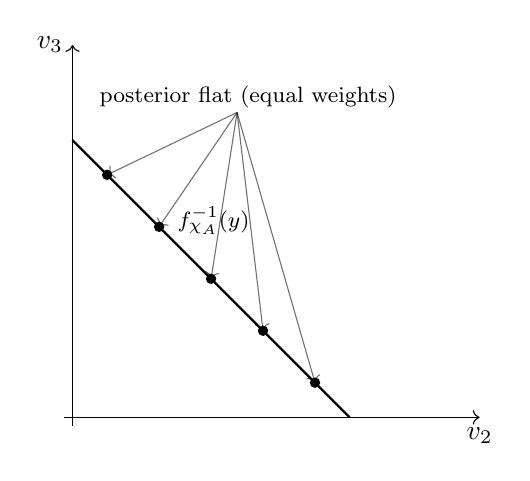
\begin{tikzpicture}[scale=2.2]
      \draw[->] (-0.05,0) -- (2.35,0) node[below] {$v_2$};
      \draw[->] (0,-0.05) -- (0,2.15) node[left] {$v_3$};
      \draw[thick] (0,1.6) -- (1.6,0);
      \node[above right] at (0.55,1.00) {\footnotesize $f_{\chi_A}^{-1}(y)$};
      \foreach \t in {0.2,0.5,0.8,1.1,1.4} {
        \fill (\t, {1.6-\t}) circle (0.03);
      }
      \node[anchor=west] at (0.10,1.85) {\footnotesize posterior flat (equal weights)};
      \foreach \t in {0.2,0.5,0.8,1.1,1.4} {
        \draw[->, thin, opacity=0.55] (0.95,1.76) -- (\t, {1.6-\t});
      }
    \end{tikzpicture}
    \end{minipage}
    \hfill
    \begin{minipage}[t]{0.48\textwidth}
    \centering
    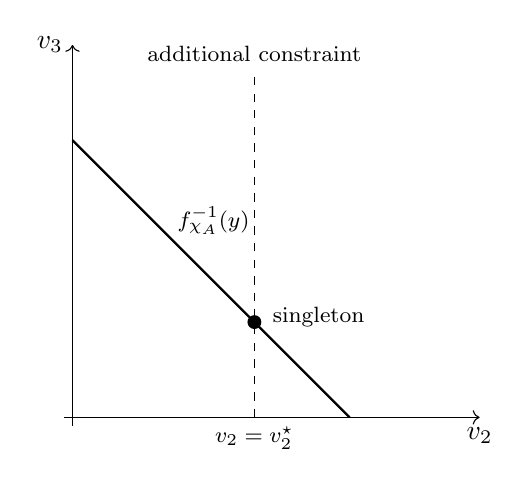
\begin{tikzpicture}[scale=2.2]
      \draw[->] (-0.05,0) -- (2.35,0) node[below] {$v_2$};
      \draw[->] (0,-0.05) -- (0,2.15) node[left] {$v_3$};
      \draw[thick] (0,1.6) -- (1.6,0);
      \node[above right] at (0.55,1.00) {\footnotesize $f_{\chi_A}^{-1}(y)$};
      \draw[dashed] (1.05,0) -- (1.05,2.0);
      \node[above] at (1.05,2.0) {\footnotesize additional constraint};
      \node[below] at (1.05,0) {\footnotesize $v_2=v_2^\star$};
      \fill (1.05,0.55) circle (0.04);
      \node[right] at (1.10,0.58) {\footnotesize singleton};
    \end{tikzpicture}
    \end{minipage}
    \caption{DSDP ($A=\{\mathrm{Alice}\}$), Layer~2 (geometric intuition in the $(v_2,v_3)$-plane): fixing the revealed output $Y=y$ selects a congruence constraint (drawn as a line).
    Left: posterior flatness means the posterior mass is uniform across the solutions in that fiber.
    Right: an additional constraint (e.g.\ learning $v_2$ under a larger corruption set) intersects the fiber and can collapse it to a singleton, breaking Layer~2.}
    \label{fig:dsdp-alice-layer2}
    \end{figure}

    \item[\textbf{$\pi_{\{\mathrm{Alice},\mathrm{Bob}\}}:E\to B_{\{\mathrm{Alice},\mathrm{Bob}\}}$ and $\pi_{\{\mathrm{Alice},\mathrm{Charlie}\}}:E\to B_{\{\mathrm{Alice},\mathrm{Charlie}\}}$.}]
    \textbf{MPC fact (operational).} Alice learns $S$ and additionally learns $v_2$ (or $v_3$) via corruption.
    \textbf{Information-geometric interpretation (Layer~2 collapse under stronger corruption).}
    Given $S$ and Alice's known $(u_1,u_2,u_3,v_1)$, the compatible set is the congruence fiber
    \[
    \mathcal{F}_S=\{(v_2,v_3):\ u_2v_2+u_3v_3=S-u_1v_1\}.
    \]
    If $u_3\neq 0$, then additionally knowing $v_2$ makes $v_3$ unique (and symmetrically if $u_2\neq 0$ and $v_3$ is known), so the fiber intersection becomes a singleton: Layer~2 can fail for these larger $A$.

    \item[\textbf{$\pi_{\{\mathrm{Alice},\mathrm{Bob},\mathrm{Charlie}\}}:E\to B_{\mathrm{full}}$ (full corruption).}]
    \textbf{MPC fact (operational).} The adversary sees all local values, hence all inputs.
    \textbf{Information-geometric interpretation.} The kernel becomes fully separating; both Layer~1 and Layer~2 are vacuous in this maximal corruption regime.
\end{description}

\subsection{SMC-SPP (\texorpdfstring{$\pi_2$}{pi2}) in the Kernel-to-Simplex Language}
\label{subsec:protocol-smc-spp}
This subsection treats Protocol~$\pi_2$ (SMC-SPP) in the same style: we model one execution as a point in a total space $E$, specify view maps $\pi_A:E\to B_A$, and interpret Layer~1/Layer~2 security as geometric statements about the induced kernels into probability simplices.

\subsubsection{Protocol model in the $E\to B$ language}
Fix a finite field $\F_q$.
Party $P_1$ holds $x_1\in\F_q$ and party $P_2$ holds $x_2\in\F_q$.
There is a \emph{commodity server} (preprocessing functionality) that samples
\[
s_1,s_2,r_1 \xleftarrow{\$} \F_q,\qquad r_2 := s_1s_2-r_1,
\]
and sends $(s_1,r_1)$ to $P_1$ and $(s_2,r_2)$ to $P_2$.
During the online phase, $P_2$ samples an output-share mask $y_2\xleftarrow{\$}\F_q$.
The protocol produces additive output shares $(y_1,y_2)\in \F_q^2$ satisfying
\[
y_1+y_2 = x_1x_2.
\]

In the ``total space'' notation, we take one execution state as
\[
E:=\bigl(x_1,x_2,s_1,s_2,r_1,y_2\bigr)\in \F_q^{6},
\]
with $r_2=s_1s_2-r_1$ treated as a derived coordinate.
The protocol transcript consists of the exchanged masked messages
\[
\hat x_1 := x_1+s_1,\qquad \hat x_2:=x_2+s_2,\qquad
t := \hat x_1\cdot x_2 + r_2 - y_2,
\]
and the local computation at $P_1$
\[
y_1 := t - \hat x_2\cdot s_1 + r_1.
\]

\subsubsection{Arrow-by-arrow map (specialized)}
\begin{description}
    \item[\textbf{$\pi_{\mathrm{out}}:E\to \F_q^2$ (output shares).}]
    \textbf{MPC fact (operational).} The protocol outputs $(y_1,y_2)$ such that $y_1+y_2=x_1x_2$.
    \textbf{Information-geometric interpretation.} The reconstruction map
    \[
    \rho:\F_q^2\to \F_q,\qquad \rho(y_1,y_2)=y_1+y_2,
    \]
    is deterministic post-processing; thus any divergence between share-laws cannot increase when mapped to the reconstructed output law (data processing).

    \item[\textbf{$\pi_{\mathrm{full}}:E\to B_{\mathrm{full}}$ (full transcript bundle).}]
    \textbf{MPC fact (counterfactual operational model).} A maximal observer records all local inputs, preprocessing deliveries, all exchanged messages $(\hat x_1,\hat x_2,t)$, and both output shares $(y_1,y_2)$.
    \textbf{Information-geometric interpretation.} This is the reference object for a corruption filtration: each concrete adversary view space $B_A$ is obtained by post-processing/projection $B_{\mathrm{full}}\to B_A$.

    \item[\textbf{$\pi_{P_1}:E\to B_{P_1}$ (view of $P_1$).}]
    \textbf{MPC fact (operational).} $P_1$ sees $(x_1)$, receives $(s_1,r_1)$ from the server, receives $\hat x_2=x_2+s_2$ from $P_2$, receives $t$ from $P_2$, and outputs $y_1$.
    \textbf{Information-geometric interpretation (Layer~1 as kernel constancy).}
    Condition on $P_1$'s fixed inputs $(x_1,s_1,r_1)$.
    Then $\hat x_2=x_2+s_2$ is uniform on $\F_q$ and independent of $x_2$ because $s_2\xleftarrow{\$}\F_q$ is uniform.
    Also $y_1=x_1x_2-y_2$ is uniform and independent of $x_1x_2$ because $y_2\xleftarrow{\$}\F_q$ is uniform.
    Hence the kernel $x_2\mapsto \mathrm{Law}(\pi_{P_1}\mid x_1,s_1,r_1)$ is constant (perfect Layer~1 for $A=\{P_1\}$).

    \item[\textbf{$\pi_{P_2}:E\to B_{P_2}$ (view of $P_2$).}]
    \textbf{MPC fact (operational).} $P_2$ sees $(x_2)$, receives $(s_2,r_2)$ from the server, receives $\hat x_1=x_1+s_1$ from $P_1$, samples $y_2\xleftarrow{\$}\F_q$, sends $t$ to $P_1$, and outputs $y_2$.
    \textbf{Information-geometric interpretation (Layer~1 as kernel constancy).}
    Conditioning on $(x_2,s_2,r_2)$, the message $\hat x_1=x_1+s_1$ is uniform and independent of $x_1$ because $s_1$ is uniform, and $y_2$ is uniform by construction.
    Hence the kernel $x_1\mapsto \mathrm{Law}(\pi_{P_2}\mid x_2,s_2,r_2)$ is constant (perfect Layer~1 for $A=\{P_2\}$).

    \item[\textbf{$\pi_{\mathrm{srv}}:E\to B_{\mathrm{srv}}$ (commodity server state).}]
    \textbf{MPC fact (operational preprocessing).} The server samples $(s_1,s_2,r_1)$ and determines $r_2=s_1s_2-r_1$.
    \textbf{Information-geometric interpretation.} Including $\mathrm{srv}$ in the corruption set enlarges $B_A$ and can make the induced kernel more separating.
    For example, $\{P_1\}\subseteq \{P_1,\mathrm{srv}\}$ lets an adversary learn both $s_2$ (from the server) and $\hat x_2$ (from the transcript), hence recover $x_2=\hat x_2-s_2$ and therefore the product $x_1x_2$.

    \item[\textbf{$\rho:\F_q^2\to \F_q$ (reconstruction).}]
    \textbf{MPC fact (operational).} If an adversary learns both shares (e.g.\ $A=\{P_1,P_2\}$), it can compute $y=x_1x_2=\rho(y_1,y_2)$.
    \textbf{Information-geometric interpretation (broken Layer~1 / output-revealing).}
    In that regime, the induced map into the output simplex becomes clustered/indexed by the output value:
    \[
    (x_1,x_2)\ \longmapsto\ \delta_{x_1x_2}\ \in\ \Prob(\F_q),
    \]
    i.e.\ the image sits on simplex vertices and distinct outputs are maximally separated (TV $=1$ for different vertices).

    \item[\textbf{Output fiber $\mathcal{F}_y\subseteq \F_q^2$ (Layer~2 constraint set).}]
    \textbf{MPC fact (structural constraint).} Fixing the revealed output $y$ constrains inputs to $\mathcal{F}_y=\{(x_1,x_2):x_1x_2=y\}$.
    \textbf{Information-geometric interpretation (Layer~2).}
    Under a uniform prior on $(x_1,x_2)$, the max-entropy/I-projection posterior is uniform on $\mathcal{F}_y$ (Definition~\ref{def:layer2}; compare Section~\ref{subsec:kl-projection-principles}).
    \emph{Corruption caveat:} if the adversary also knows $x_1$ (resp.\ $x_2$) and $x_1\neq 0$ (resp.\ $x_2\neq 0$), then the fiber intersected with that constraint is a singleton, so Layer~2 non-triviality can fail.
\end{description}

\section{Appendix: Visual toy examples on the \texorpdfstring{$2$}{2}-simplex (three-outcome views)}
\label{app:visual-toy-simplex}

The main body uses the simplex language \emph{abstractly}: kernels map hidden coordinates to points in a simplex $\Prob(B_A)$, and leakage corresponds to separation of these points (diameter in TV/KL, sensitivity via Fisher, etc.).
This appendix provides self-contained toy constructions in the smallest nontrivial case
\[
B_A^{\mathrm{toy}}=\{L,C,R\},\qquad \Prob(B_A^{\mathrm{toy}})\cong \Delta^2.
\]
These examples are \emph{not} claims about any specific MPC protocol; they are visualization templates.
In practice, one obtains a three-outcome alphabet by \emph{coarse-graining} a rich transcript $B_A\to \{L,C,R\}$ (bucket two events of interest and group all other outcomes into a final category), and then plotting the induced view laws for different secrets/inputs.
Equivalently, if $g:B_A\to\{L,C,R\}$ is the bucketing map and $Q_x\in\Prob(B_A)$ is a true view law (conditioned on a hidden coordinate $x$), then the plotted toy law is the pushforward $g_\# Q_x\in\Prob(\{L,C,R\})\cong \Delta^2$.
The triangle drawings are Euclidean embeddings used only for visualization: straight segments correspond to \emph{mixtures} (affine geometry), while the I-projection is defined by KL minimization (not Euclidean orthogonality).

\subsection{Toy MPC-style view kernel into \texorpdfstring{$\Delta^2$}{Delta2} (two secrets; three outcomes)}
\label{subsec:toy-kernel-delta2}

Let the hidden coordinate be a one-bit ``secret'' $X\in\{0,1\}$ and let the adversary's (coarse-grained) view alphabet be $B_A^{\mathrm{toy}}=\{L,C,R\}$.
Suppose the induced conditional view laws are
\[
p_0:=\mathrm{Law}(V_A\mid X=0)=(0.6,0.3,0.1),\qquad
p_1:=\mathrm{Law}(V_A\mid X=1)=(0.1,0.3,0.6),
\]
written in the coordinate order $(L,C,R)$.
Then the map $x\mapsto p_x$ is a law-valued kernel $\{0,1\}\to\Delta^2$.
Perfect Layer~1 for this coarse-grained view would be $p_0=p_1$ (collapse to a point in $\Delta^2$); leakage corresponds to separation between $p_0$ and $p_1$ (e.g.\ in TV/KL).

\begin{figure}[ht]
\centering
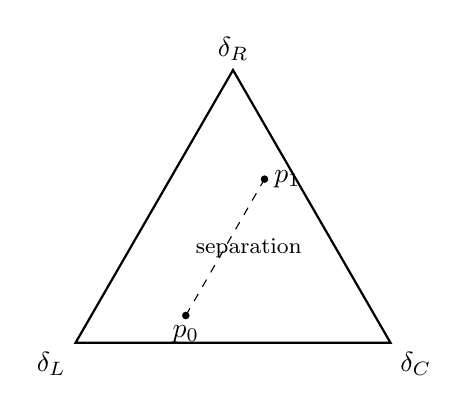
\begin{tikzpicture}[scale=4]
  % Vertices of the standard 2-simplex in R^2
  \coordinate (L) at (0,0);
  \coordinate (C) at (1,0);
  \coordinate (R) at (0.5,0.866);

  % Two example points: p0=(0.6,0.3,0.1), p1=(0.1,0.3,0.6)
  % Map (pL,pC,pR) to Euclidean coords: pL*L + pC*C + pR*R
  \coordinate (p0) at (0.35,0.0866);
  \coordinate (p1) at (0.60,0.5196);

  \draw[thick] (L) -- (C) -- (R) -- cycle;

  \node[below left]  at (L) {$\delta_L$};
  \node[below right] at (C) {$\delta_C$};
  \node[above]       at (R) {$\delta_R$};

  \fill (p0) circle (0.012);
  \fill (p1) circle (0.012);
  \node[below] at (p0) {$p_0$};
  \node[right] at (p1) {$p_1$};

  \draw[dashed] (p0) -- (p1);
  \node at (0.55,0.30) {\footnotesize separation};
\end{tikzpicture}
\caption{A three-outcome simplex $\Delta^2$ with two induced view laws $p_0,p_1$. Collapse (perfect Layer~1) would mean $p_0=p_1$.}
\label{fig:toy-kernel-delta2}
\end{figure}

\subsection{Mixture model of leakage (a line segment in the simplex)}
\label{subsec:toy-mixture-leakage}

A convenient way to get literal line segments (mixture geometry) is to write the view law as a mixture of an ``ideal'' (secret-independent) component and a ``leaky'' component.
Let $u=(1/3,1/3,1/3)$ be the uniform distribution on $B_A^{\mathrm{toy}}$, and let the extreme leaky laws be $\delta_L$ and $\delta_R$.
For a leakage parameter $\theta\in[0,1]$, define
\[
p^{(\theta)}_0 := (1-\theta)u + \theta\,\delta_L,\qquad
p^{(\theta)}_1 := (1-\theta)u + \theta\,\delta_R.
\]
As $\theta$ increases, the two points move along straight-line mixture segments from the center $u$ to opposite vertices, making the geometric meaning of ``more leakage'' literal in $\Delta^2$.

\begin{figure}[ht]
\centering
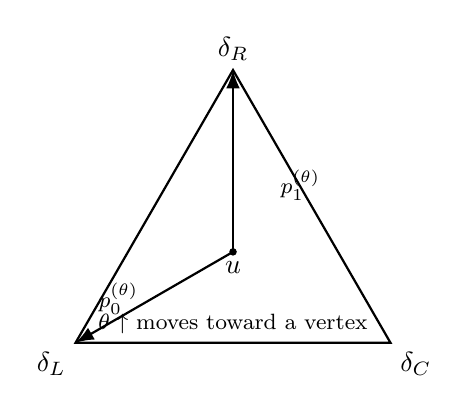
\begin{tikzpicture}[scale=4]
  \coordinate (L) at (0,0);
  \coordinate (C) at (1,0);
  \coordinate (R) at (0.5,0.866);
  \draw[thick] (L) -- (C) -- (R) -- cycle;

  % u=(1/3,1/3,1/3) -> (0.5, 0.2887)
  \coordinate (u) at (0.5,0.2887);

  \fill (u) circle (0.012);
  \node[below] at (u) {$u$};

  \node[below left]  at (L) {$\delta_L$};
  \node[below right] at (C) {$\delta_C$};
  \node[above]       at (R) {$\delta_R$};

  \draw[thick,{-Latex}] (u) -- (L);
  \draw[thick,{-Latex}] (u) -- (R);
  \node[left]  at (0.23,0.14) {\footnotesize $p^{(\theta)}_0$};
  \node[right] at (0.62,0.50) {\footnotesize $p^{(\theta)}_1$};

  \node at (0.50,0.06) {\footnotesize $\theta\uparrow$ moves toward a vertex};
\end{tikzpicture}
\caption{A toy mixture-leakage model: $\theta$ moves the induced laws along mixture line segments from a secret-independent center $u$ toward secret-dependent vertices.}
\label{fig:toy-mixture-lines}
\end{figure}

\subsection{An I-projection ``picture'' (constraint slice + max-entropy completion)}
\label{subsec:toy-i-projection-picture}

To visualize I-projection/max-entropy geometry, fix a baseline distribution and impose a constraint that cuts out an affine slice of the simplex.
Let the baseline be $q=u=(1/3,1/3,1/3)$ and define a statistic $T:B_A^{\mathrm{toy}}\to\R$ by
\[
T(L)=0,\qquad T(C)=1,\qquad T(R)=2.
\]
For a target moment $t\in(0,2)$, consider the constraint set
\[
\mathcal{C}_t:=\{p\in\Delta^2:\ \mathbb{E}_p[T]=t\}.
\]
This is an affine line segment inside the triangle (because $\mathbb{E}_p[T]=p_C+2p_R$ in these coordinates).
The \textbf{I-projection} (equivalently, max-entropy completion relative to a uniform baseline) is
\[
p^\star\in \arg\min_{p\in \mathcal{C}_t} D_{\mathrm{KL}}(p\|u).
\]
In this finite-alphabet setting, $p^\star$ has an exponential-family form:
\[
p^\star(L)=\frac{1}{Z(\lambda)},\quad
p^\star(C)=\frac{e^\lambda}{Z(\lambda)},\quad
p^\star(R)=\frac{e^{2\lambda}}{Z(\lambda)},\qquad
Z(\lambda)=1+e^\lambda+e^{2\lambda},
\]
where $\lambda$ is chosen so that $\mathbb{E}_{p^\star}[T]=t$.
For example, at $t=1.3$ one finds $\lambda\approx 0.5$ and $p^\star\approx (0.186,0.307,0.507)$.

\begin{figure}[ht]
\centering
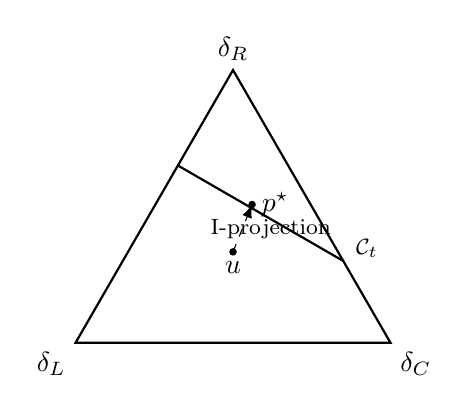
\begin{tikzpicture}[scale=4]
  \coordinate (L) at (0,0);
  \coordinate (C) at (1,0);
  \coordinate (R) at (0.5,0.866);
  \draw[thick] (L) -- (C) -- (R) -- cycle;

  % Baseline u=(1/3,1/3,1/3)
  \coordinate (u) at (0.5,0.2887);
  \fill (u) circle (0.012);
  \node[below] at (u) {$u$};

  % Constraint E[T]=t with t=1.3: pC+2 pR=1.3 intersects simplex at:
  % A: (pL,pC,pR)=(0.35,0,0.65) -> (0.325,0.5629)
  % B: (0,0.7,0.3) -> (0.85,0.2598)
  \coordinate (A) at (0.325,0.5629);
  \coordinate (B) at (0.85,0.2598);
  \draw[thick] (A) -- (B);
  \node[right] at (0.86,0.30) {\footnotesize $\mathcal{C}_{t}$};

  % Example I-projection point p* ~ (0.186,0.307,0.507) -> (0.5605,0.439)
  \coordinate (pstar) at (0.5605,0.439);
  \fill (pstar) circle (0.012);
  \node[right] at (pstar) {$p^\star$};

  \draw[dashed,{-Latex}] (u) -- (pstar);
  \node at (0.62,0.36) {\footnotesize I-projection};

  \node[below left]  at (L) {$\delta_L$};
  \node[below right] at (C) {$\delta_C$};
  \node[above]       at (R) {$\delta_R$};
\end{tikzpicture}
\caption{A constraint slice $\mathcal{C}_t=\{p:\mathbb{E}_p[T]=t\}$ inside $\Delta^2$ and the I-projection/max-entropy completion $p^\star$ of a baseline $u$ onto that slice (drawn as an arrow; the projection is in KL geometry, not Euclidean).}
\label{fig:toy-i-projection}
\end{figure}

\paragraph{How to use this in real protocol examples.}
To get a drawable picture from a complicated transcript alphabet $B_A$:
(i) choose a coarse-graining $B_A\to\{L,C,R\}$ (three events/buckets),
(ii) compute/estimate the induced laws $p(\cdot\mid x)$ or $p_{\theta}(\cdot\mid x)$,
and (iii) interpret separation/motion/constraints using Figures~\ref{fig:toy-kernel-delta2}--\ref{fig:toy-i-projection} as templates.
This does not replace a proof, but it provides an honest geometric visualization of kernels into simplices.

\end{document}

